% =====================================================================
%  MODEL CARDS  --  % =====================================================================
%  MODEL CARDS  --  % =====================================================================
%  MODEL CARDS  --  % =====================================================================
%  MODEL CARDS  --  \input{models_frames} from 2_presentation.tex
%
%  Every card carries the same four things in the same order:
%     ALGORITHM  --  what it is, by name
%     EQUATION   --  what the code computes
%     DIAGRAM    --  the mechanism, drawn
%     MEASURED   --  a number from this repository
%
%  HEIGHT BUDGET -- READ THIS BEFORE ADDING A LINE.
%  A 16:9 frame gives ~6.8cm of body once title, subtitle and footline
%  are paid for. That is about 20 lines at \scriptsize, 27 at \tiny.
%  A display equation \[..\] costs ~3 lines.
%
%  Every card carries [shrink=15]: beamer measures the frame and scales
%  it down ONLY if it would overflow, up to 15%. A frame that already
%  fits is untouched. This is a SAFETY NET, not a licence to overfill --
%  past 15% the content runs off the bottom edge silently, exactly as it
%  did before. If you add an equation, delete a bullet to pay for it.
%
%  Overleaf prints "Overfull \vbox" for any frame that needed shrinking;
%  that warning is the signal to cut a line, not to raise the 15%.
%
%  All figures measured from the repository, 14 Sep 2026.
% =====================================================================

% ---------------------------------------------------------------------
\begin{frame}[shrink=15]{2. Model Inventory --- Five Scoring Heads and One Gate}
\framesubtitle{Each is a different model class, defined where the others are not}
\vspace{1mm}
\begin{center}
{\scriptsize
\renewcommand{\arraystretch}{1.22}
\begin{tabular}{c L{2.5cm} L{3.9cm} c c c}
\toprule
\textbf{Head} & \textbf{Model class} & \textbf{What it computes} & \textbf{Range} & \textbf{Cov.} & \textbf{Wt.}\\
\midrule
$S_{\mathit{sem}}$     & Transformer encoder   & Cosine to a 384-d sentence embedding & $[-1,1]$ & \textbf{100\%} & $1.00$\\
$S_{\mathit{graph}}$   & Graph neural net (CF) & Inner product of LightGCN embeddings & $[-1,1]$ & \textcolor{amritaMaroon}{\textbf{0.20\%}} & $0.20$\\
$S_{\mathit{ema}}$     & Online moving average & Cosine to the live user vector       & $[-1,1]$ & \textbf{100\%} & $0.15$\\
$S_{\mathit{kg}}$      & Set overlap, 0 params & Query / entity token overlap         & $[0,1]$  & \textbf{100\%} & $0.08$\\
$S_{\mathit{profile}}$ & Weighted term matcher & Declared-profile alignment           & $[-1,1]$ & \textbf{100\%} & $0.10$\\
\midrule
\textit{gate} & \textit{Hard predicate} & \textit{May this viewer see this item at all?} & $\{0,1\}$ & \textbf{100\%} & \textit{---}\\
\bottomrule
\end{tabular}}
\end{center}
\vspace{1mm}
{\scriptsize
\[ S(q,u,i) = S_{\mathit{sem}} + 0.20\,S_{\mathit{graph}} + 0.15\,S_{\mathit{ema}} + 0.08\,S_{\mathit{kg}} + 0.10\,S_{\mathit{profile}} \]}
\vspace{-3mm}
{\scriptsize\textbf{Why coverage is the column that matters.} The graph head is our strongest signal
and is defined for \textbf{0.20\%} of the catalog; every other head is defined everywhere. That is
why the blend is additive with a dominant semantic term rather than a learned gate --- a missing
head must degrade the ranking, never break it.}
\end{frame}

% ---------------------------------------------------------------------
\begin{frame}[shrink=15]{2. Model 1 --- SBERT Semantic Encoder}
\framesubtitle{Algorithm $\cdot$ equation $\cdot$ measured result}
\vspace{1mm}
\begin{center}
  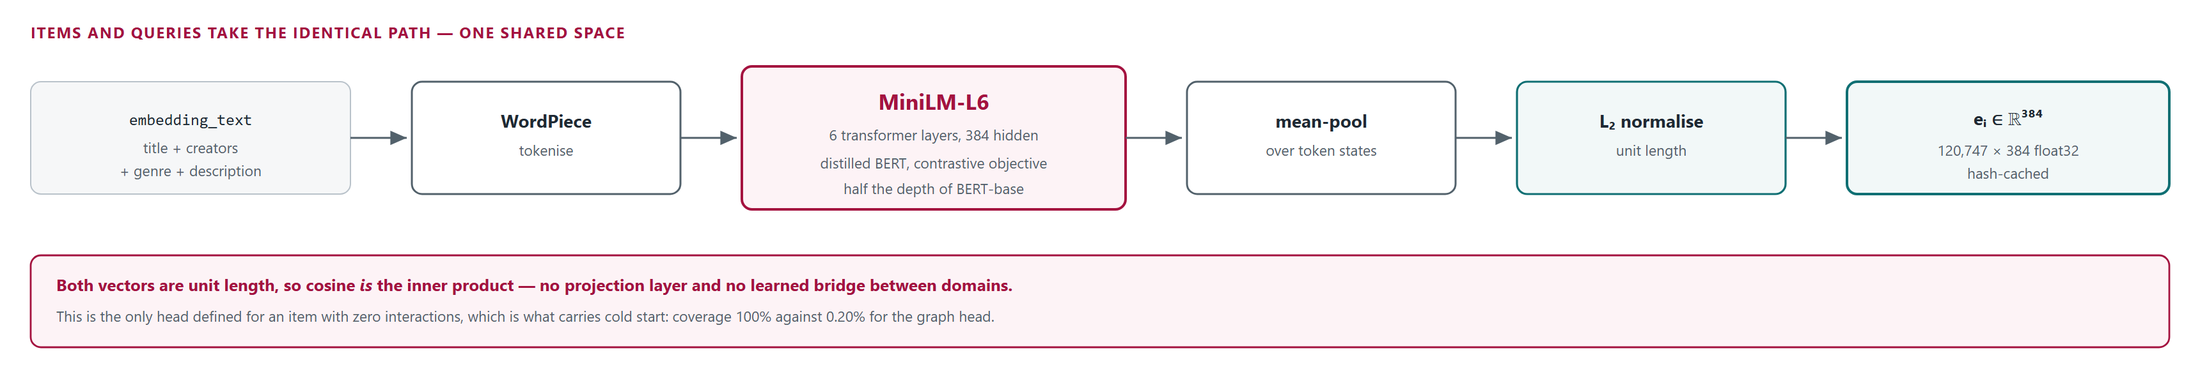
\includegraphics[width=\linewidth,height=3.4cm,keepaspectratio]{sbert}
\end{center}
\vspace{2mm}
\begin{columns}[T]
\column{0.485\textwidth}
\blk{Algorithm and equation}
{\scriptsize \texttt{all-MiniLM-L6-v2} --- a 6-layer distilled BERT, mean pooling over token states.
\[ \mathbf{e}_i = \frac{\mathrm{MeanPool}(\mathrm{MiniLM}(t_i))}{\lVert\cdot\rVert_2}, \quad
   S_{\mathit{sem}} = \mathbf{e}_i^{\top}\mathbf{q} \]
Both vectors are unit length, so cosine \emph{is} the inner product. The query takes the identical
path --- one shared space, no projection layer.}

\column{0.485\textwidth}
\blk{Measured}
\begin{tight}
  \item \textbf{120{,}747 $\times$ 384} float32; batch 256; hash-cached, so only changed rows
        re-encode.
  \item \textbf{Coverage 100\%} --- the only head defined at zero interactions, which is what
        carries cold start.
  \item 6 layers not 12, so the catalog encodes in one GPU pass and serving stays CPU-only.
\end{tight}
\end{columns}
\end{frame}

% ---------------------------------------------------------------------
\begin{frame}[shrink=15]{2. Model 2 --- LightGCN Graph Collaborative Filtering}
\framesubtitle{Algorithm $\cdot$ equation $\cdot$ measured result}
\vspace{1mm}
\begin{columns}[T]
\column{0.45\textwidth}
\blk{Algorithm}
{\scriptsize LightGCN (He et al., SIGIR 2020) --- a \emph{linear} convolution on the user--item
bipartite graph. Unlike NGCF there is \textbf{no feature transform and no nonlinearity}; the only
learned parameters are the layer-0 embeddings.}
\vspace{1.5mm}

\blk{Equations, as implemented}
{\scriptsize
With $\tilde{A} = D^{-1/2} A D^{-1/2}$, propagate and take the layer mean:
\[ \mathbf{E}^{(\ell)} = \tilde{A}\mathbf{E}^{(\ell-1)}, \quad
   \mathbf{E} = \tfrac{1}{L+1}\textstyle\sum_{\ell=0}^{L}\mathbf{E}^{(\ell)} \]
Score, and train by the BPR pairwise objective:
\[ \hat y_{ui} = \mathbf{e}_u^{\top}\mathbf{e}_i \]
\[ \mathcal{L} = -\!\sum \ln\sigma(\hat y_{ui}-\hat y_{uj}) + \lambda\lVert\mathbf{E}^{(0)}\rVert^2 \]}
\vspace{-1mm}
{\tiny\textbf{Config:} $d{=}64$, $L{=}3$, lr $10^{-3}$, decay $10^{-4}$, batch \textbf{4096},
60 epochs, seed 42, Kaggle T4.}

\column{0.52\textwidth}
\blk{Measured --- against a popularity control}
{\tiny
\renewcommand{\arraystretch}{1.15}
\begin{tabular}{L{1.4cm} l c c c c}
\toprule
\textbf{Domain} & \textbf{Model} & \textbf{R@20} & \textbf{N@20} & \textbf{MRR} & \textbf{Lift}\\
\midrule
Movies \& TV & LightGCN & \textbf{0.0288} & \textbf{0.0125} & \textbf{0.0080} & \\
             & popular  & 0.0182 & 0.0080 & 0.0052 & \textbf{1.59$\times$}\\
\midrule
Industrial   & LightGCN & \textbf{0.0326} & \textbf{0.0138} & \textbf{0.0087} & \\
             & popular  & 0.0264 & 0.0111 & 0.0070 & \textbf{1.24$\times$}\\
\midrule
Health       & LightGCN & 0.0121 & 0.0046 & 0.0025 & \\
             & popular  & \textbf{0.0221} & \textbf{0.0093} & \textbf{0.0059} & \textcolor{amritaMaroon}{\textbf{0.55$\times$}}\\
\bottomrule
\end{tabular}}\\[1.5mm]
{\tiny\textbf{Protocol.} Ratings $\geq 4$ as implicit positives; 10-core (Industrial keeps the
source 5-core floor); leave-last-out; 49{,}958 / 33{,}929 / 50{,}000 users evaluated.}\\[1.5mm]
{\tiny\textbf{$\mathtt{recall}=\mathtt{hit\_rate}$ is correct, not a bug:} leave-last-out gives one
relevant item, so Recall@$K \equiv$ HitRate@$K$. Check: $0.0288/20 = 0.00144$.}\\[1.5mm]
{\tiny\textcolor{amritaMaroon}{\textbf{Health regresses.}} BPR trains on the raw inner product, but
evaluation and serving both $L_2$-normalise and rank by cosine --- dividing by the \emph{item} norm
is not rank-preserving, and that norm carries the popularity prior.}
\end{columns}
\end{frame}

% ---------------------------------------------------------------------
%  PANEL RECOMMENDATION 1 -- NCF: position, architecture and plan
% ---------------------------------------------------------------------
\begin{frame}[shrink=15]{2. Panel Recommendation --- Neural Collaborative Filtering}
\framesubtitle{What NCF is, how it differs from LightGCN, and how we will test it}
\vspace{1mm}
\begin{columns}[T]
\column{0.475\textwidth}
\blk{What the panel asked for}
{\scriptsize NCF (He et al., WWW 2017) replaces the \emph{fixed} inner product with a \emph{learned}
similarity. NeuMF runs two towers and fuses them:
\[ \hat y^{\mathit{GMF}} = \mathbf{p}_u \odot \mathbf{q}_i, \quad
   \hat y^{\mathit{MLP}} = \phi_L(\cdots\phi_1([\mathbf{p}'_u \| \mathbf{q}'_i])) \]
\[ \hat y_{ui} = \sigma\big(\mathbf{h}^{\top}[\,\hat y^{\mathit{GMF}} \,\|\, \hat y^{\mathit{MLP}}\,]\big) \]
The MLP tower models \textbf{non-linear} interaction --- which our inner product cannot.}
\vspace{1.5mm}

\blk{How it differs from what we run}
\begin{tight}
  \item \textbf{LightGCN is graph-based:} it propagates over the bipartite graph, so a user is
        informed by items three hops away. \textbf{NCF has no graph} --- it learns a similarity on
        ids alone. They are complementary, not substitutes.
\end{tight}

\column{0.495\textwidth}
\vspace{-2mm}
\begin{center}
  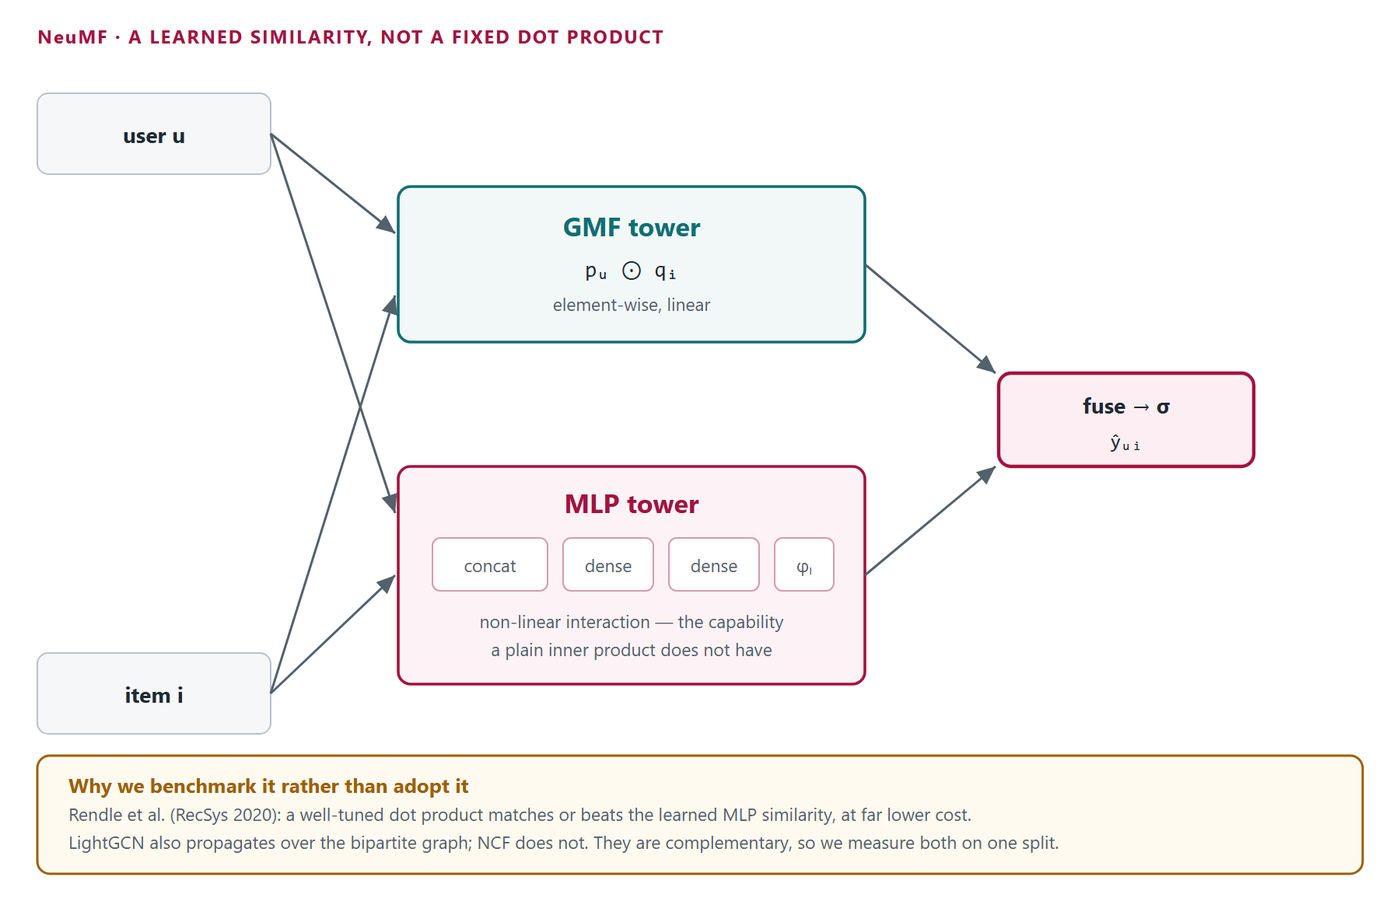
\includegraphics[width=\linewidth,height=4.9cm,keepaspectratio]{ncf}
\end{center}
\vspace{1mm}

\blk{Our position, and the plan}
\begin{tight}
  \item Rendle et al.\ (RecSys 2020) revisited this comparison and found a \textbf{well-tuned dot
        product matches or beats} the learned MLP, at far lower cost --- so we will run NeuMF as a
        \emph{measured baseline}, not adopt it as an assumed upgrade.
  \item The harness already runs three domains on fixed splits, so NeuMF slots in behind the same
        interface; then report popularity / LightGCN / NeuMF side by side.
\end{tight}
\end{columns}
\end{frame}

% ---------------------------------------------------------------------
\begin{frame}[shrink=15]{2. Model 3 --- Real-Time EMA User Vector}
\framesubtitle{Algorithm $\cdot$ equation $\cdot$ measured result}
\vspace{1mm}
\begin{columns}[T]
\column{0.515\textwidth}
\blk{Algorithm}
{\scriptsize A \textbf{signed, strength-scaled} exponential moving average in the same 384-d space
as the items. Not a plain average: a negative event pushes the user vector \emph{away} from the
item, and the step scales with how strong the event was.}
\vspace{1.5mm}

\blk{Equations, as implemented}
{\scriptsize
Event weight $w$: $+1.2$ complete, $+1.0$ like, $+0.6$ click, $+0.4$ view, $-1.0$ skip; a rating
$v$ maps to $(v-3)/2$. Then with $\alpha = 0.25$:
\[ d=\operatorname{sign}(w),\ \ s=\min(|w|,1),\ \ \eta=\operatorname{clip}(\alpha s,0,1) \]
\[ \mathbf{u}_{t+1} = \frac{(1-\eta)\mathbf{u}_t + \eta\,d\,\mathbf{e}_i}{\lVert\cdot\rVert_2},
   \ \ S_{\mathit{ema}} = \mathbf{u}_t^{\top}\mathbf{e}_i \]}

\column{0.46\textwidth}
\vspace{-3mm}
\begin{center}
  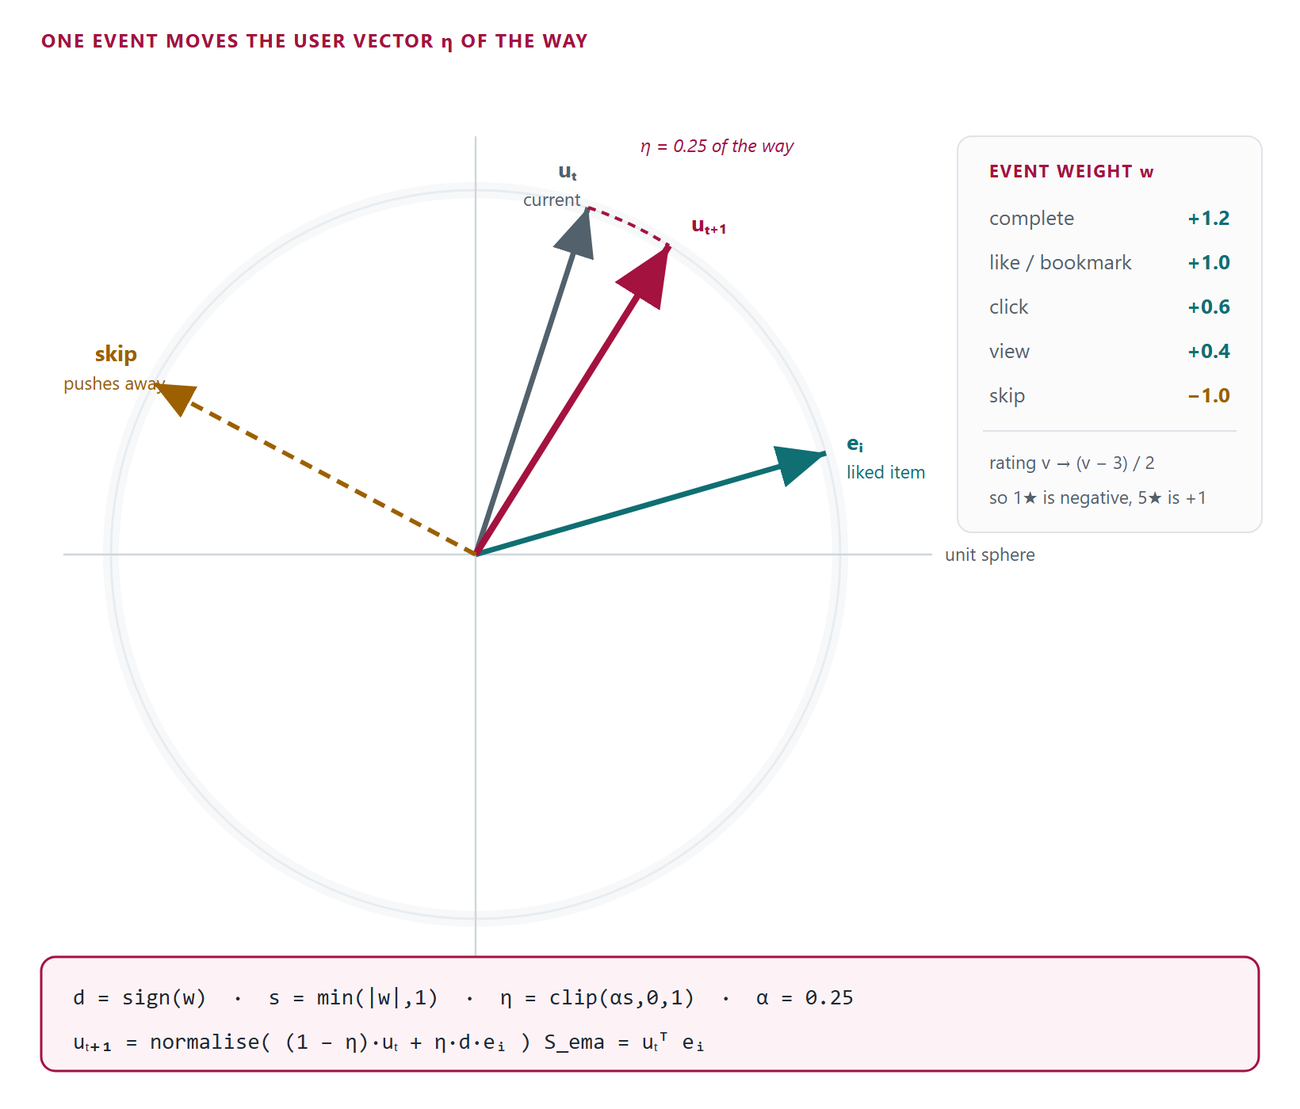
\includegraphics[width=\linewidth,height=5.5cm,keepaspectratio]{ema}
\end{center}
\vspace{1mm}

\blk{Measured}
\begin{tight}
  \item \textbf{39.0\,$\mu$s} per update, \textbf{16.7\,$\mu$s} per score (1{,}000 ops, 384-d).
  \item Against \textbf{hours} for a retrain --- five orders of magnitude. This is the "real-time"
        in the project title, as a number.
  \item \textbf{Limitation:} no session boundary or time decay, so one misclick persists.
\end{tight}
\end{columns}
\end{frame}

% ---------------------------------------------------------------------
\begin{frame}[shrink=15]{2. Model 4 --- Knowledge-Graph Overlap Head}
\framesubtitle{Algorithm $\cdot$ equation $\cdot$ measured result}
\vspace{1mm}
\begin{columns}[T]
\column{0.47\textwidth}
\blk{Algorithm and equation}
{\scriptsize A \textbf{zero-parameter set-overlap scorer} over shared entity namespaces. Nothing is
trained, so nothing drifts --- and it is defined precisely where the graph model is not. With
$T(i)$ the token set over \{title, description, creators, categories, type\}:
\[ S_{\mathit{kg}} = \min\!\left(1,\ \frac{|T(q)\cap T(i)|}{\max(3,|T(q)|)}\right) \]
The $\max(3,\cdot)$ floor stops a one-word query scoring 1.0 on one incidental match.}
\vspace{1.5mm}

\blk{Measured}
\begin{tight}
  \item Mean \textbf{KG@5 $=$ 0.892} over 8 scenarios; \textbf{0.667} on both named-entity queries,
        where dense retrieval smears.
  \item \textbf{Coverage 100\%} --- it reads metadata, not behaviour.
\end{tight}

\column{0.50\textwidth}
\vspace{-3mm}
\begin{center}
  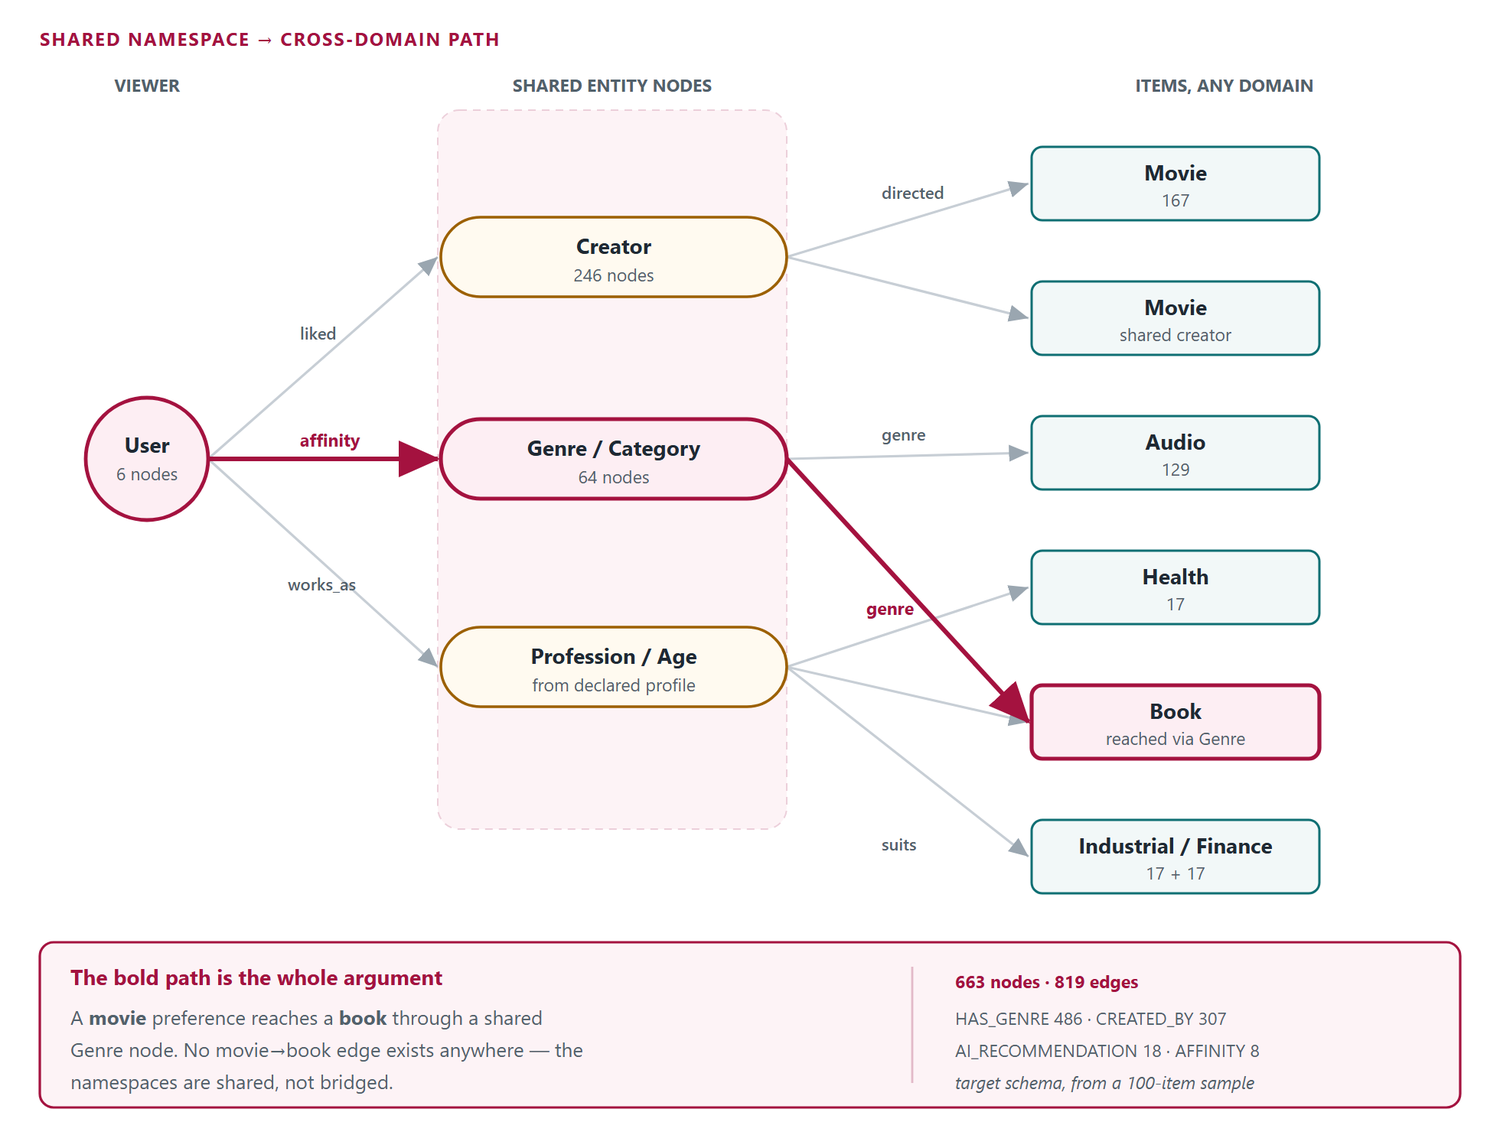
\includegraphics[width=\linewidth,height=5.7cm,keepaspectratio]{kg}
\end{center}
\vspace{1mm}

{\scriptsize\textcolor{amritaMaroon}{\textbf{Bold path:}} a \emph{movie} preference reaches a
\emph{book} through a shared Genre node --- no movie-to-book edge exists anywhere.}\\[1mm]
{\tiny\textbf{Scope.} At request time this is the overlap function above; the 663-node figure is the
\emph{target schema} from a 100-item example, not a runtime graph. Neo4j is Review 3.}
\end{columns}
\end{frame}

% ---------------------------------------------------------------------
\begin{frame}[shrink=15]{2. Model 5 --- Profile Head and the Eligibility Gate}
\framesubtitle{Algorithm $\cdot$ equation $\cdot$ measured result}
\vspace{1mm}
\begin{columns}[T]
\column{0.53\textwidth}
\blk{Profile head --- a score}
{\footnotesize A \textbf{weighted term matcher} against the declared profile; avoid-terms subtract
at nearly twice the weight of a positive match.
\[ S_{\mathit{profile}} = \operatorname{clip}\big(0.16|P\cap i| - 0.25|A\cap i| + 0.15\cdot\mathbf{1}[\tau_i \in \Pi]\big) \]}
\vspace{-3mm}
{\scriptsize $P$ = interests $\cup$ likes $\cup$ skills $\cup$ role $\cup$ age terms; \ $A$ = avoid
terms; \ $\Pi$ = preferred types; clipped to $[-1,1]$.}
\vspace{3mm}

\blk{Eligibility --- a predicate, not a score}
{\footnotesize
\[ \mathrm{elig}(i\,|\,c) = \mathbf{1}\big[a_{\mathit{eff}} \geq \mathrm{minage}(i)\big] \wedge \mathbf{1}\big[\tau_i \in \mathcal{T}(d)\big] \]
Compiled \emph{into} the Qdrant query, so an ineligible item is never retrieved, never scored, and
cannot be promoted back by any head.}
\vspace{2mm}

{\footnotesize\textbf{Fail-closed.} No age supplied caps at teen, not adult. Unknown metadata falls
back to the content-type default, never to unrestricted. Health and finance are \textbf{discovery
only, never advice}.}

\column{0.445\textwidth}
\vspace{-2mm}
\begin{center}
  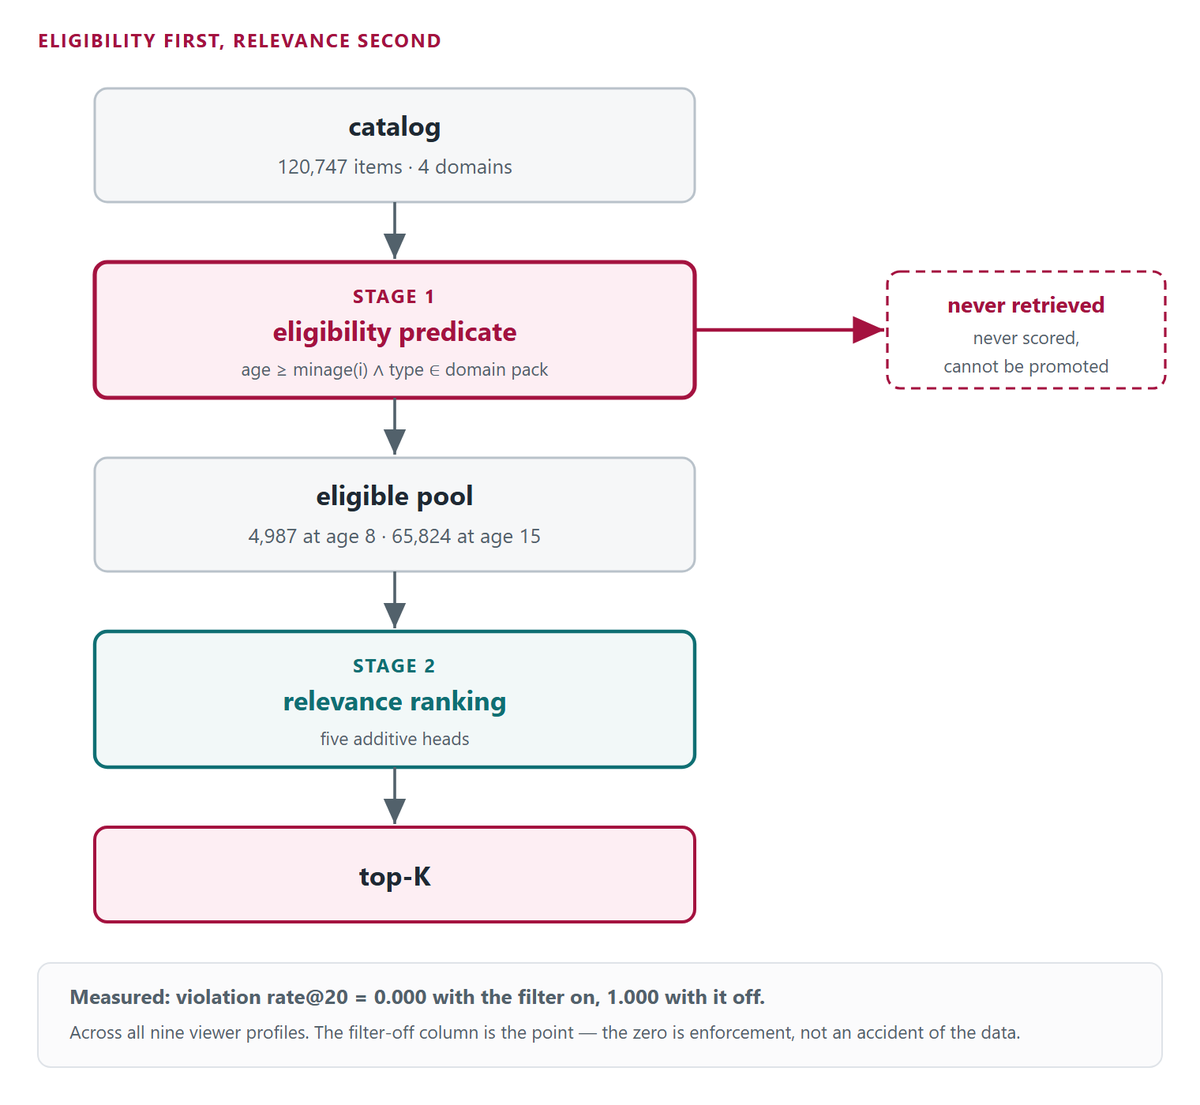
\includegraphics[width=\linewidth,height=5.9cm,keepaspectratio]{gate}
\end{center}
\vspace{2mm}
\blk{Measured}
\begin{tight}
  \item Mean \textbf{profile@5 $=$ 0.957}; \textbf{8 of 8} scenarios fully profile-positive.
  \item Violations \textbf{0.000} on, \textbf{1.000} off, across \textbf{9} viewer profiles.
\end{tight}
\end{columns}
\end{frame}
 from 2_presentation.tex
%
%  Every card carries the same four things in the same order:
%     ALGORITHM  --  what it is, by name
%     EQUATION   --  what the code computes
%     DIAGRAM    --  the mechanism, drawn
%     MEASURED   --  a number from this repository
%
%  HEIGHT BUDGET -- READ THIS BEFORE ADDING A LINE.
%  A 16:9 frame gives ~6.8cm of body once title, subtitle and footline
%  are paid for. That is about 20 lines at \scriptsize, 27 at \tiny.
%  A display equation \[..\] costs ~3 lines.
%
%  Every card carries [shrink=15]: beamer measures the frame and scales
%  it down ONLY if it would overflow, up to 15%. A frame that already
%  fits is untouched. This is a SAFETY NET, not a licence to overfill --
%  past 15% the content runs off the bottom edge silently, exactly as it
%  did before. If you add an equation, delete a bullet to pay for it.
%
%  Overleaf prints "Overfull \vbox" for any frame that needed shrinking;
%  that warning is the signal to cut a line, not to raise the 15%.
%
%  All figures measured from the repository, 14 Sep 2026.
% =====================================================================

% ---------------------------------------------------------------------
\begin{frame}[shrink=15]{2. Model Inventory --- Five Scoring Heads and One Gate}
\framesubtitle{Each is a different model class, defined where the others are not}
\vspace{1mm}
\begin{center}
{\scriptsize
\renewcommand{\arraystretch}{1.22}
\begin{tabular}{c L{2.5cm} L{3.9cm} c c c}
\toprule
\textbf{Head} & \textbf{Model class} & \textbf{What it computes} & \textbf{Range} & \textbf{Cov.} & \textbf{Wt.}\\
\midrule
$S_{\mathit{sem}}$     & Transformer encoder   & Cosine to a 384-d sentence embedding & $[-1,1]$ & \textbf{100\%} & $1.00$\\
$S_{\mathit{graph}}$   & Graph neural net (CF) & Inner product of LightGCN embeddings & $[-1,1]$ & \textcolor{amritaMaroon}{\textbf{0.20\%}} & $0.20$\\
$S_{\mathit{ema}}$     & Online moving average & Cosine to the live user vector       & $[-1,1]$ & \textbf{100\%} & $0.15$\\
$S_{\mathit{kg}}$      & Set overlap, 0 params & Query / entity token overlap         & $[0,1]$  & \textbf{100\%} & $0.08$\\
$S_{\mathit{profile}}$ & Weighted term matcher & Declared-profile alignment           & $[-1,1]$ & \textbf{100\%} & $0.10$\\
\midrule
\textit{gate} & \textit{Hard predicate} & \textit{May this viewer see this item at all?} & $\{0,1\}$ & \textbf{100\%} & \textit{---}\\
\bottomrule
\end{tabular}}
\end{center}
\vspace{1mm}
{\scriptsize
\[ S(q,u,i) = S_{\mathit{sem}} + 0.20\,S_{\mathit{graph}} + 0.15\,S_{\mathit{ema}} + 0.08\,S_{\mathit{kg}} + 0.10\,S_{\mathit{profile}} \]}
\vspace{-3mm}
{\scriptsize\textbf{Why coverage is the column that matters.} The graph head is our strongest signal
and is defined for \textbf{0.20\%} of the catalog; every other head is defined everywhere. That is
why the blend is additive with a dominant semantic term rather than a learned gate --- a missing
head must degrade the ranking, never break it.}
\end{frame}

% ---------------------------------------------------------------------
\begin{frame}[shrink=15]{2. Model 1 --- SBERT Semantic Encoder}
\framesubtitle{Algorithm $\cdot$ equation $\cdot$ measured result}
\vspace{1mm}
\begin{center}
  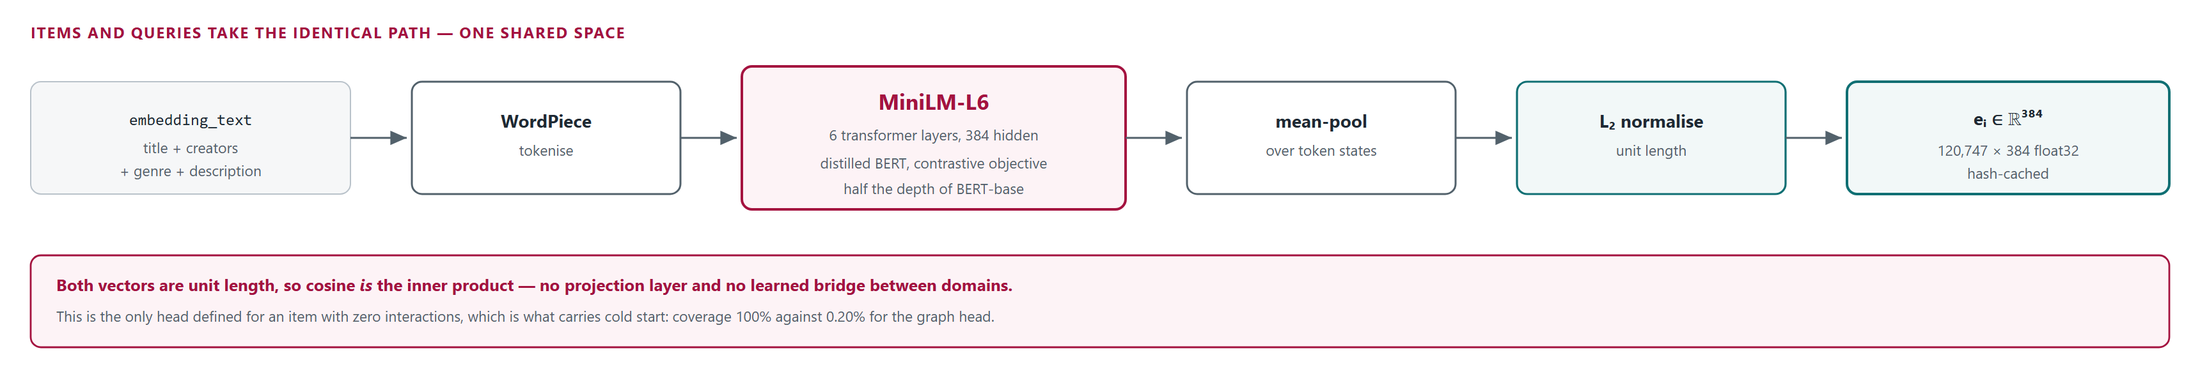
\includegraphics[width=\linewidth,height=3.4cm,keepaspectratio]{sbert}
\end{center}
\vspace{2mm}
\begin{columns}[T]
\column{0.485\textwidth}
\blk{Algorithm and equation}
{\scriptsize \texttt{all-MiniLM-L6-v2} --- a 6-layer distilled BERT, mean pooling over token states.
\[ \mathbf{e}_i = \frac{\mathrm{MeanPool}(\mathrm{MiniLM}(t_i))}{\lVert\cdot\rVert_2}, \quad
   S_{\mathit{sem}} = \mathbf{e}_i^{\top}\mathbf{q} \]
Both vectors are unit length, so cosine \emph{is} the inner product. The query takes the identical
path --- one shared space, no projection layer.}

\column{0.485\textwidth}
\blk{Measured}
\begin{tight}
  \item \textbf{120{,}747 $\times$ 384} float32; batch 256; hash-cached, so only changed rows
        re-encode.
  \item \textbf{Coverage 100\%} --- the only head defined at zero interactions, which is what
        carries cold start.
  \item 6 layers not 12, so the catalog encodes in one GPU pass and serving stays CPU-only.
\end{tight}
\end{columns}
\end{frame}

% ---------------------------------------------------------------------
\begin{frame}[shrink=15]{2. Model 2 --- LightGCN Graph Collaborative Filtering}
\framesubtitle{Algorithm $\cdot$ equation $\cdot$ measured result}
\vspace{1mm}
\begin{columns}[T]
\column{0.45\textwidth}
\blk{Algorithm}
{\scriptsize LightGCN (He et al., SIGIR 2020) --- a \emph{linear} convolution on the user--item
bipartite graph. Unlike NGCF there is \textbf{no feature transform and no nonlinearity}; the only
learned parameters are the layer-0 embeddings.}
\vspace{1.5mm}

\blk{Equations, as implemented}
{\scriptsize
With $\tilde{A} = D^{-1/2} A D^{-1/2}$, propagate and take the layer mean:
\[ \mathbf{E}^{(\ell)} = \tilde{A}\mathbf{E}^{(\ell-1)}, \quad
   \mathbf{E} = \tfrac{1}{L+1}\textstyle\sum_{\ell=0}^{L}\mathbf{E}^{(\ell)} \]
Score, and train by the BPR pairwise objective:
\[ \hat y_{ui} = \mathbf{e}_u^{\top}\mathbf{e}_i \]
\[ \mathcal{L} = -\!\sum \ln\sigma(\hat y_{ui}-\hat y_{uj}) + \lambda\lVert\mathbf{E}^{(0)}\rVert^2 \]}
\vspace{-1mm}
{\tiny\textbf{Config:} $d{=}64$, $L{=}3$, lr $10^{-3}$, decay $10^{-4}$, batch \textbf{4096},
60 epochs, seed 42, Kaggle T4.}

\column{0.52\textwidth}
\blk{Measured --- against a popularity control}
{\tiny
\renewcommand{\arraystretch}{1.15}
\begin{tabular}{L{1.4cm} l c c c c}
\toprule
\textbf{Domain} & \textbf{Model} & \textbf{R@20} & \textbf{N@20} & \textbf{MRR} & \textbf{Lift}\\
\midrule
Movies \& TV & LightGCN & \textbf{0.0288} & \textbf{0.0125} & \textbf{0.0080} & \\
             & popular  & 0.0182 & 0.0080 & 0.0052 & \textbf{1.59$\times$}\\
\midrule
Industrial   & LightGCN & \textbf{0.0326} & \textbf{0.0138} & \textbf{0.0087} & \\
             & popular  & 0.0264 & 0.0111 & 0.0070 & \textbf{1.24$\times$}\\
\midrule
Health       & LightGCN & 0.0121 & 0.0046 & 0.0025 & \\
             & popular  & \textbf{0.0221} & \textbf{0.0093} & \textbf{0.0059} & \textcolor{amritaMaroon}{\textbf{0.55$\times$}}\\
\bottomrule
\end{tabular}}\\[1.5mm]
{\tiny\textbf{Protocol.} Ratings $\geq 4$ as implicit positives; 10-core (Industrial keeps the
source 5-core floor); leave-last-out; 49{,}958 / 33{,}929 / 50{,}000 users evaluated.}\\[1.5mm]
{\tiny\textbf{$\mathtt{recall}=\mathtt{hit\_rate}$ is correct, not a bug:} leave-last-out gives one
relevant item, so Recall@$K \equiv$ HitRate@$K$. Check: $0.0288/20 = 0.00144$.}\\[1.5mm]
{\tiny\textcolor{amritaMaroon}{\textbf{Health regresses.}} BPR trains on the raw inner product, but
evaluation and serving both $L_2$-normalise and rank by cosine --- dividing by the \emph{item} norm
is not rank-preserving, and that norm carries the popularity prior.}
\end{columns}
\end{frame}

% ---------------------------------------------------------------------
%  PANEL RECOMMENDATION 1 -- NCF: position, architecture and plan
% ---------------------------------------------------------------------
\begin{frame}[shrink=15]{2. Panel Recommendation --- Neural Collaborative Filtering}
\framesubtitle{What NCF is, how it differs from LightGCN, and how we will test it}
\vspace{1mm}
\begin{columns}[T]
\column{0.475\textwidth}
\blk{What the panel asked for}
{\scriptsize NCF (He et al., WWW 2017) replaces the \emph{fixed} inner product with a \emph{learned}
similarity. NeuMF runs two towers and fuses them:
\[ \hat y^{\mathit{GMF}} = \mathbf{p}_u \odot \mathbf{q}_i, \quad
   \hat y^{\mathit{MLP}} = \phi_L(\cdots\phi_1([\mathbf{p}'_u \| \mathbf{q}'_i])) \]
\[ \hat y_{ui} = \sigma\big(\mathbf{h}^{\top}[\,\hat y^{\mathit{GMF}} \,\|\, \hat y^{\mathit{MLP}}\,]\big) \]
The MLP tower models \textbf{non-linear} interaction --- which our inner product cannot.}
\vspace{1.5mm}

\blk{How it differs from what we run}
\begin{tight}
  \item \textbf{LightGCN is graph-based:} it propagates over the bipartite graph, so a user is
        informed by items three hops away. \textbf{NCF has no graph} --- it learns a similarity on
        ids alone. They are complementary, not substitutes.
\end{tight}

\column{0.495\textwidth}
\vspace{-2mm}
\begin{center}
  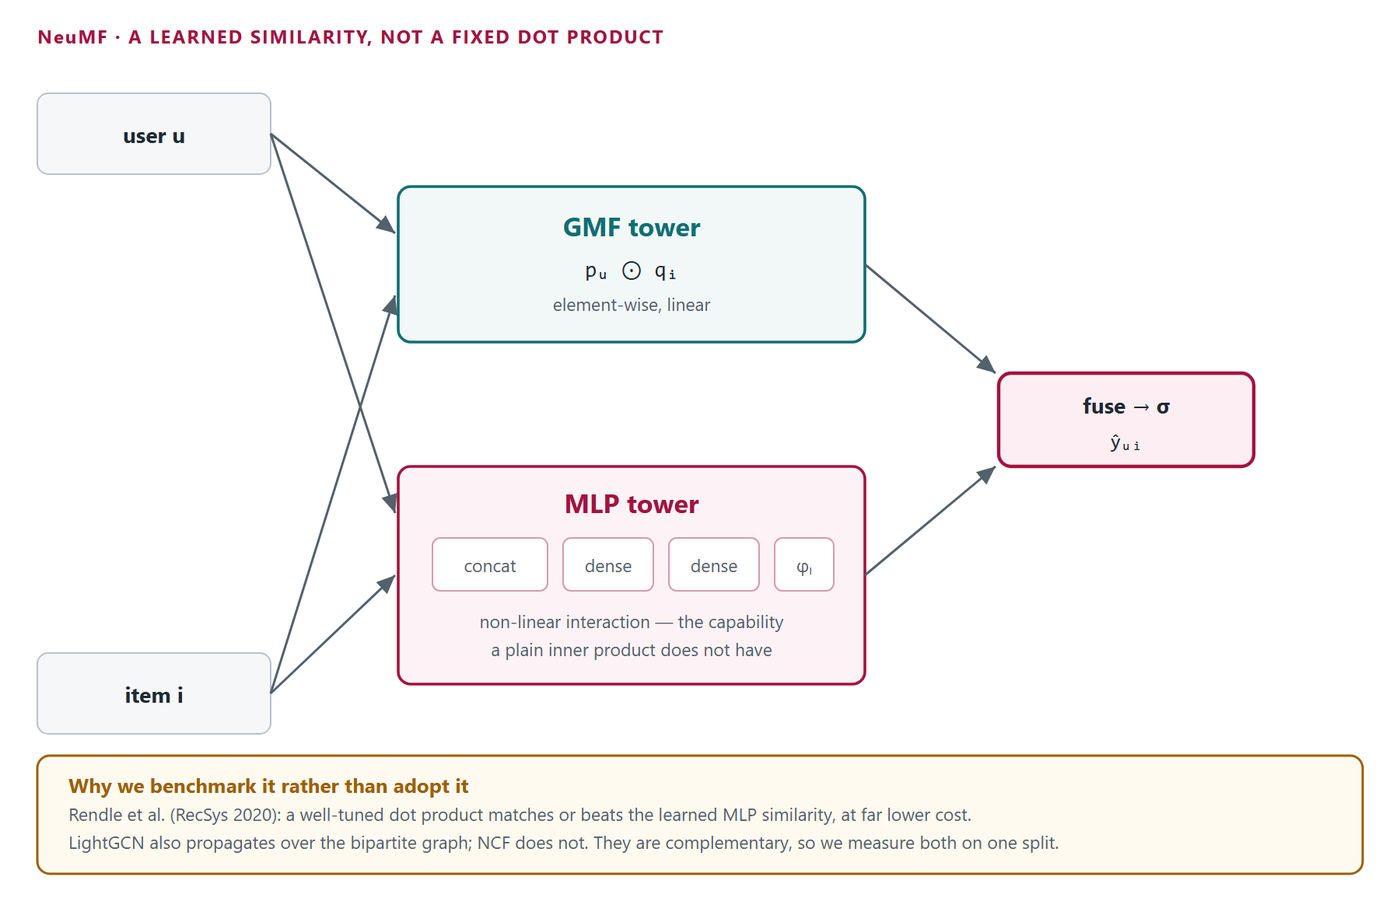
\includegraphics[width=\linewidth,height=4.9cm,keepaspectratio]{ncf}
\end{center}
\vspace{1mm}

\blk{Our position, and the plan}
\begin{tight}
  \item Rendle et al.\ (RecSys 2020) revisited this comparison and found a \textbf{well-tuned dot
        product matches or beats} the learned MLP, at far lower cost --- so we will run NeuMF as a
        \emph{measured baseline}, not adopt it as an assumed upgrade.
  \item The harness already runs three domains on fixed splits, so NeuMF slots in behind the same
        interface; then report popularity / LightGCN / NeuMF side by side.
\end{tight}
\end{columns}
\end{frame}

% ---------------------------------------------------------------------
\begin{frame}[shrink=15]{2. Model 3 --- Real-Time EMA User Vector}
\framesubtitle{Algorithm $\cdot$ equation $\cdot$ measured result}
\vspace{1mm}
\begin{columns}[T]
\column{0.515\textwidth}
\blk{Algorithm}
{\scriptsize A \textbf{signed, strength-scaled} exponential moving average in the same 384-d space
as the items. Not a plain average: a negative event pushes the user vector \emph{away} from the
item, and the step scales with how strong the event was.}
\vspace{1.5mm}

\blk{Equations, as implemented}
{\scriptsize
Event weight $w$: $+1.2$ complete, $+1.0$ like, $+0.6$ click, $+0.4$ view, $-1.0$ skip; a rating
$v$ maps to $(v-3)/2$. Then with $\alpha = 0.25$:
\[ d=\operatorname{sign}(w),\ \ s=\min(|w|,1),\ \ \eta=\operatorname{clip}(\alpha s,0,1) \]
\[ \mathbf{u}_{t+1} = \frac{(1-\eta)\mathbf{u}_t + \eta\,d\,\mathbf{e}_i}{\lVert\cdot\rVert_2},
   \ \ S_{\mathit{ema}} = \mathbf{u}_t^{\top}\mathbf{e}_i \]}

\column{0.46\textwidth}
\vspace{-3mm}
\begin{center}
  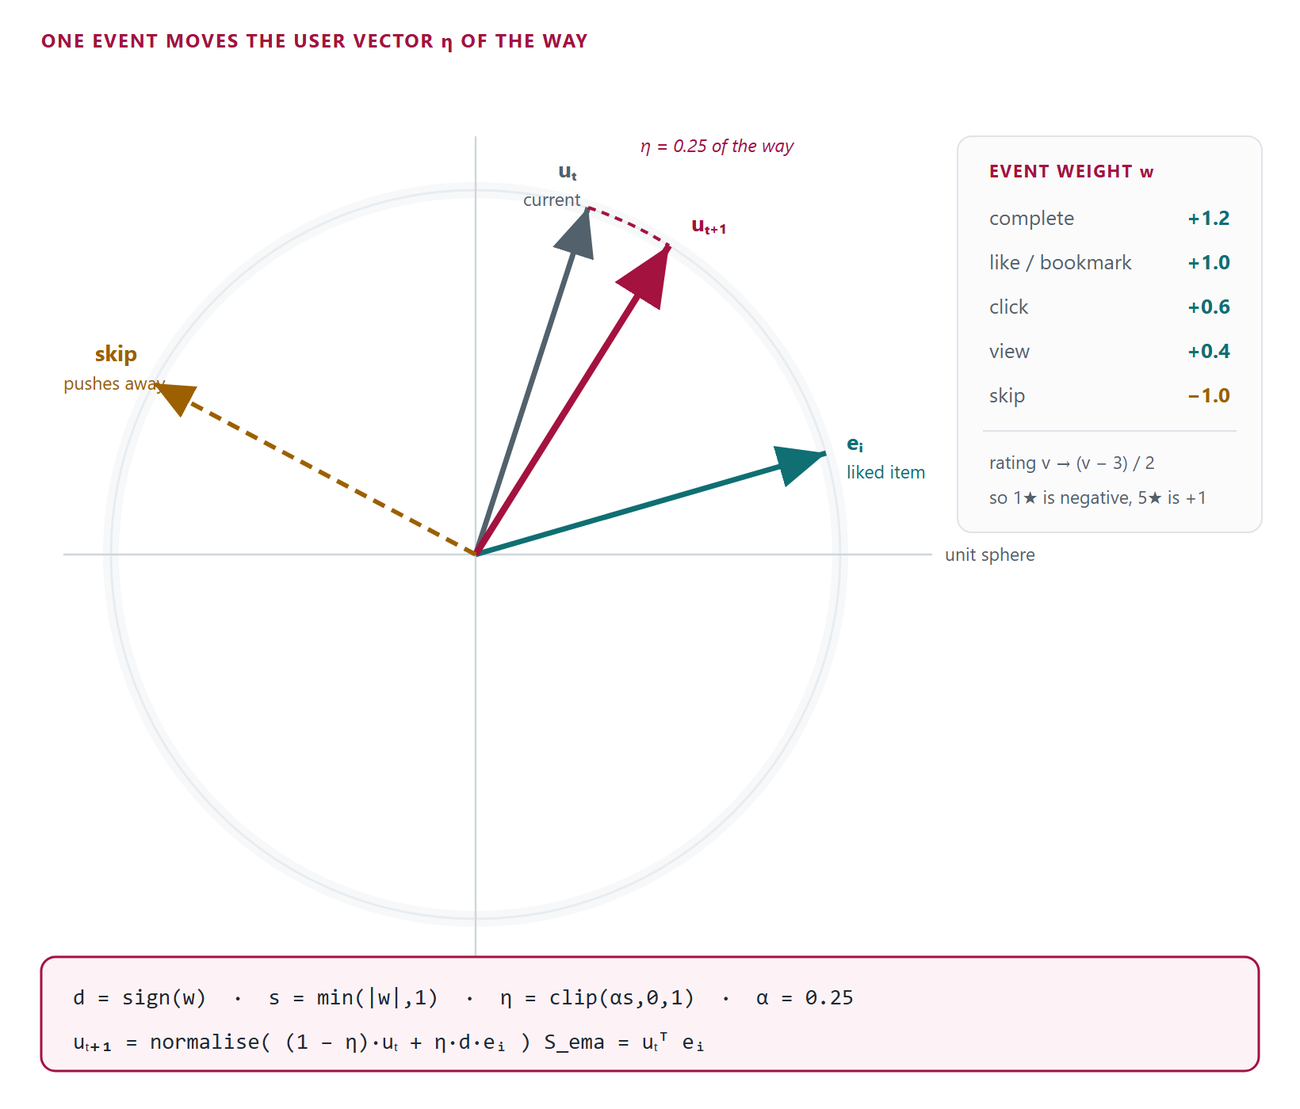
\includegraphics[width=\linewidth,height=5.5cm,keepaspectratio]{ema}
\end{center}
\vspace{1mm}

\blk{Measured}
\begin{tight}
  \item \textbf{39.0\,$\mu$s} per update, \textbf{16.7\,$\mu$s} per score (1{,}000 ops, 384-d).
  \item Against \textbf{hours} for a retrain --- five orders of magnitude. This is the "real-time"
        in the project title, as a number.
  \item \textbf{Limitation:} no session boundary or time decay, so one misclick persists.
\end{tight}
\end{columns}
\end{frame}

% ---------------------------------------------------------------------
\begin{frame}[shrink=15]{2. Model 4 --- Knowledge-Graph Overlap Head}
\framesubtitle{Algorithm $\cdot$ equation $\cdot$ measured result}
\vspace{1mm}
\begin{columns}[T]
\column{0.47\textwidth}
\blk{Algorithm and equation}
{\scriptsize A \textbf{zero-parameter set-overlap scorer} over shared entity namespaces. Nothing is
trained, so nothing drifts --- and it is defined precisely where the graph model is not. With
$T(i)$ the token set over \{title, description, creators, categories, type\}:
\[ S_{\mathit{kg}} = \min\!\left(1,\ \frac{|T(q)\cap T(i)|}{\max(3,|T(q)|)}\right) \]
The $\max(3,\cdot)$ floor stops a one-word query scoring 1.0 on one incidental match.}
\vspace{1.5mm}

\blk{Measured}
\begin{tight}
  \item Mean \textbf{KG@5 $=$ 0.892} over 8 scenarios; \textbf{0.667} on both named-entity queries,
        where dense retrieval smears.
  \item \textbf{Coverage 100\%} --- it reads metadata, not behaviour.
\end{tight}

\column{0.50\textwidth}
\vspace{-3mm}
\begin{center}
  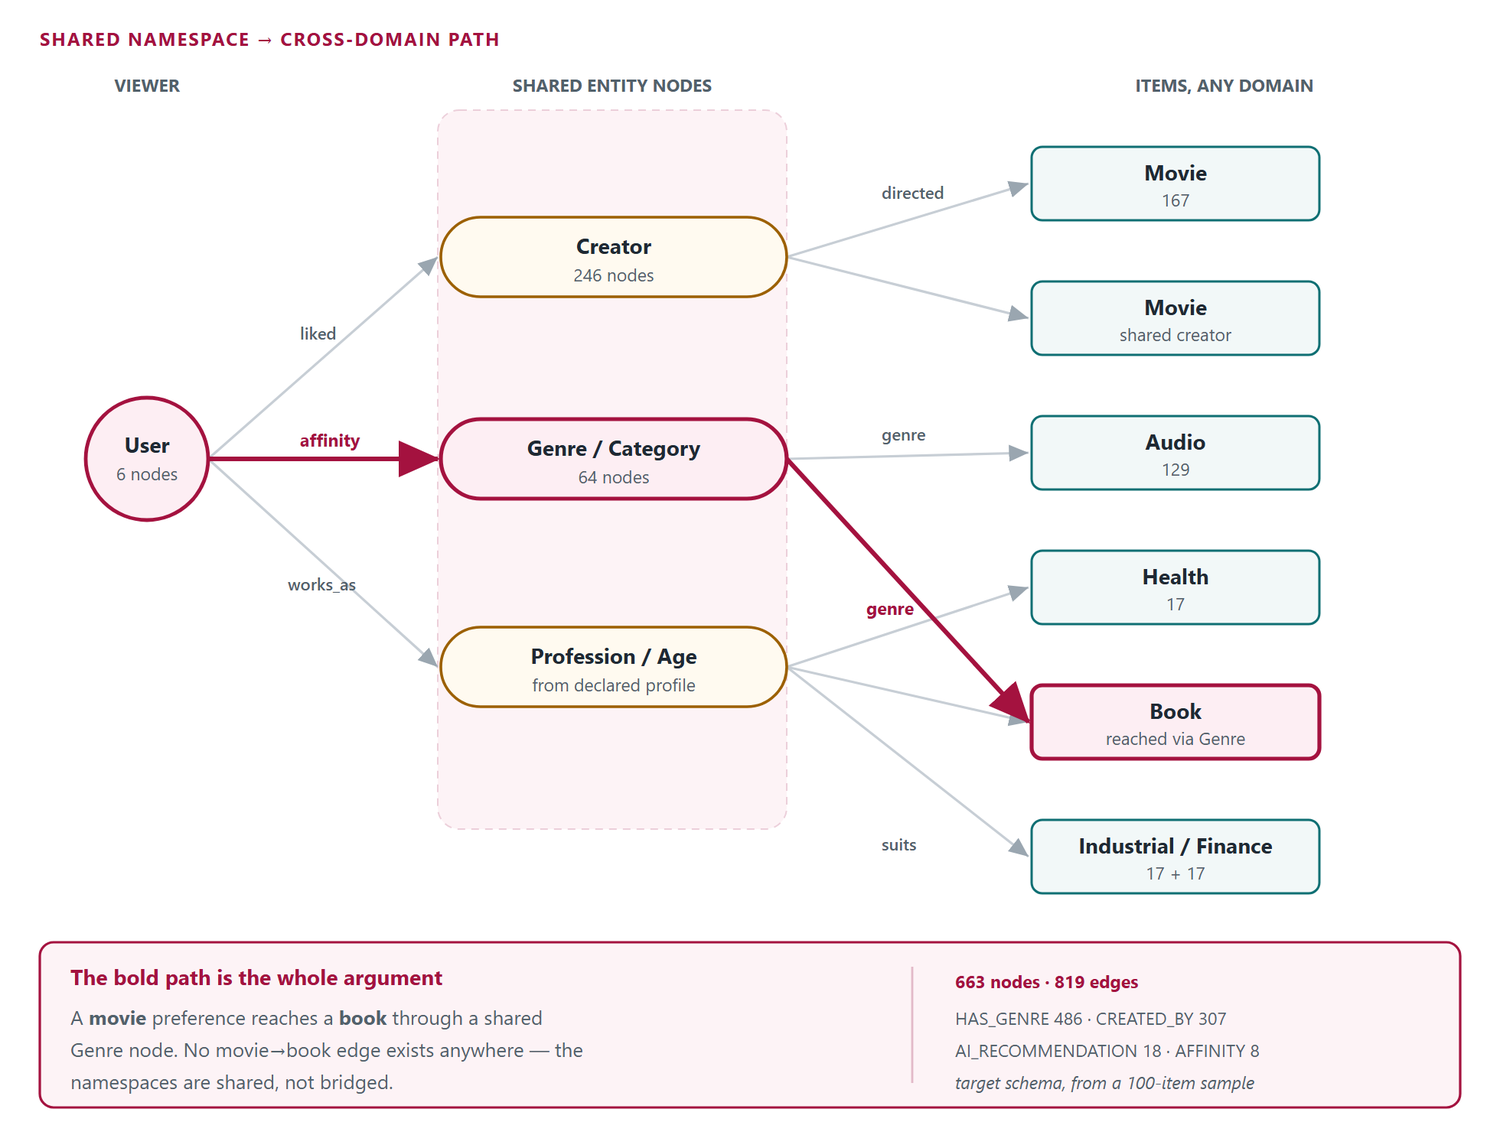
\includegraphics[width=\linewidth,height=5.7cm,keepaspectratio]{kg}
\end{center}
\vspace{1mm}

{\scriptsize\textcolor{amritaMaroon}{\textbf{Bold path:}} a \emph{movie} preference reaches a
\emph{book} through a shared Genre node --- no movie-to-book edge exists anywhere.}\\[1mm]
{\tiny\textbf{Scope.} At request time this is the overlap function above; the 663-node figure is the
\emph{target schema} from a 100-item example, not a runtime graph. Neo4j is Review 3.}
\end{columns}
\end{frame}

% ---------------------------------------------------------------------
\begin{frame}[shrink=15]{2. Model 5 --- Profile Head and the Eligibility Gate}
\framesubtitle{Algorithm $\cdot$ equation $\cdot$ measured result}
\vspace{1mm}
\begin{columns}[T]
\column{0.53\textwidth}
\blk{Profile head --- a score}
{\footnotesize A \textbf{weighted term matcher} against the declared profile; avoid-terms subtract
at nearly twice the weight of a positive match.
\[ S_{\mathit{profile}} = \operatorname{clip}\big(0.16|P\cap i| - 0.25|A\cap i| + 0.15\cdot\mathbf{1}[\tau_i \in \Pi]\big) \]}
\vspace{-3mm}
{\scriptsize $P$ = interests $\cup$ likes $\cup$ skills $\cup$ role $\cup$ age terms; \ $A$ = avoid
terms; \ $\Pi$ = preferred types; clipped to $[-1,1]$.}
\vspace{3mm}

\blk{Eligibility --- a predicate, not a score}
{\footnotesize
\[ \mathrm{elig}(i\,|\,c) = \mathbf{1}\big[a_{\mathit{eff}} \geq \mathrm{minage}(i)\big] \wedge \mathbf{1}\big[\tau_i \in \mathcal{T}(d)\big] \]
Compiled \emph{into} the Qdrant query, so an ineligible item is never retrieved, never scored, and
cannot be promoted back by any head.}
\vspace{2mm}

{\footnotesize\textbf{Fail-closed.} No age supplied caps at teen, not adult. Unknown metadata falls
back to the content-type default, never to unrestricted. Health and finance are \textbf{discovery
only, never advice}.}

\column{0.445\textwidth}
\vspace{-2mm}
\begin{center}
  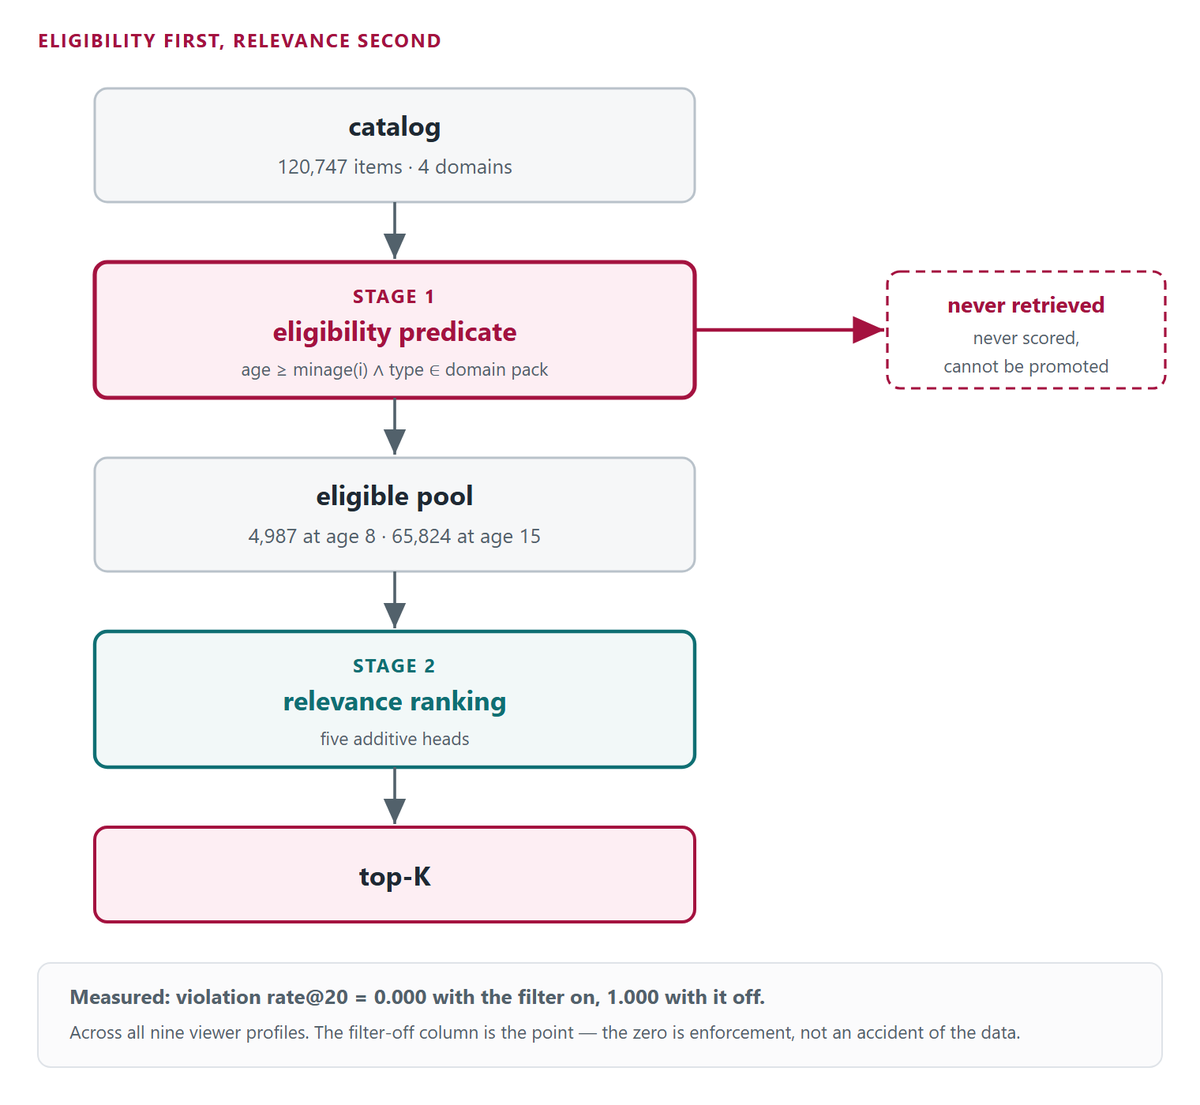
\includegraphics[width=\linewidth,height=5.9cm,keepaspectratio]{gate}
\end{center}
\vspace{2mm}
\blk{Measured}
\begin{tight}
  \item Mean \textbf{profile@5 $=$ 0.957}; \textbf{8 of 8} scenarios fully profile-positive.
  \item Violations \textbf{0.000} on, \textbf{1.000} off, across \textbf{9} viewer profiles.
\end{tight}
\end{columns}
\end{frame}
 from 2_presentation.tex
%
%  Every card carries the same four things in the same order:
%     ALGORITHM  --  what it is, by name
%     EQUATION   --  what the code computes
%     DIAGRAM    --  the mechanism, drawn
%     MEASURED   --  a number from this repository
%
%  HEIGHT BUDGET -- READ THIS BEFORE ADDING A LINE.
%  A 16:9 frame gives ~6.8cm of body once title, subtitle and footline
%  are paid for. That is about 20 lines at \scriptsize, 27 at \tiny.
%  A display equation \[..\] costs ~3 lines.
%
%  Every card carries [shrink=15]: beamer measures the frame and scales
%  it down ONLY if it would overflow, up to 15%. A frame that already
%  fits is untouched. This is a SAFETY NET, not a licence to overfill --
%  past 15% the content runs off the bottom edge silently, exactly as it
%  did before. If you add an equation, delete a bullet to pay for it.
%
%  Overleaf prints "Overfull \vbox" for any frame that needed shrinking;
%  that warning is the signal to cut a line, not to raise the 15%.
%
%  All figures measured from the repository, 14 Sep 2026.
% =====================================================================

% ---------------------------------------------------------------------
\begin{frame}[shrink=15]{2. Model Inventory --- Five Scoring Heads and One Gate}
\framesubtitle{Each is a different model class, defined where the others are not}
\vspace{1mm}
\begin{center}
{\scriptsize
\renewcommand{\arraystretch}{1.22}
\begin{tabular}{c L{2.5cm} L{3.9cm} c c c}
\toprule
\textbf{Head} & \textbf{Model class} & \textbf{What it computes} & \textbf{Range} & \textbf{Cov.} & \textbf{Wt.}\\
\midrule
$S_{\mathit{sem}}$     & Transformer encoder   & Cosine to a 384-d sentence embedding & $[-1,1]$ & \textbf{100\%} & $1.00$\\
$S_{\mathit{graph}}$   & Graph neural net (CF) & Inner product of LightGCN embeddings & $[-1,1]$ & \textcolor{amritaMaroon}{\textbf{0.20\%}} & $0.20$\\
$S_{\mathit{ema}}$     & Online moving average & Cosine to the live user vector       & $[-1,1]$ & \textbf{100\%} & $0.15$\\
$S_{\mathit{kg}}$      & Set overlap, 0 params & Query / entity token overlap         & $[0,1]$  & \textbf{100\%} & $0.08$\\
$S_{\mathit{profile}}$ & Weighted term matcher & Declared-profile alignment           & $[-1,1]$ & \textbf{100\%} & $0.10$\\
\midrule
\textit{gate} & \textit{Hard predicate} & \textit{May this viewer see this item at all?} & $\{0,1\}$ & \textbf{100\%} & \textit{---}\\
\bottomrule
\end{tabular}}
\end{center}
\vspace{1mm}
{\scriptsize
\[ S(q,u,i) = S_{\mathit{sem}} + 0.20\,S_{\mathit{graph}} + 0.15\,S_{\mathit{ema}} + 0.08\,S_{\mathit{kg}} + 0.10\,S_{\mathit{profile}} \]}
\vspace{-3mm}
{\scriptsize\textbf{Why coverage is the column that matters.} The graph head is our strongest signal
and is defined for \textbf{0.20\%} of the catalog; every other head is defined everywhere. That is
why the blend is additive with a dominant semantic term rather than a learned gate --- a missing
head must degrade the ranking, never break it.}
\end{frame}

% ---------------------------------------------------------------------
\begin{frame}[shrink=15]{2. Model 1 --- SBERT Semantic Encoder}
\framesubtitle{Algorithm $\cdot$ equation $\cdot$ measured result}
\vspace{1mm}
\begin{center}
  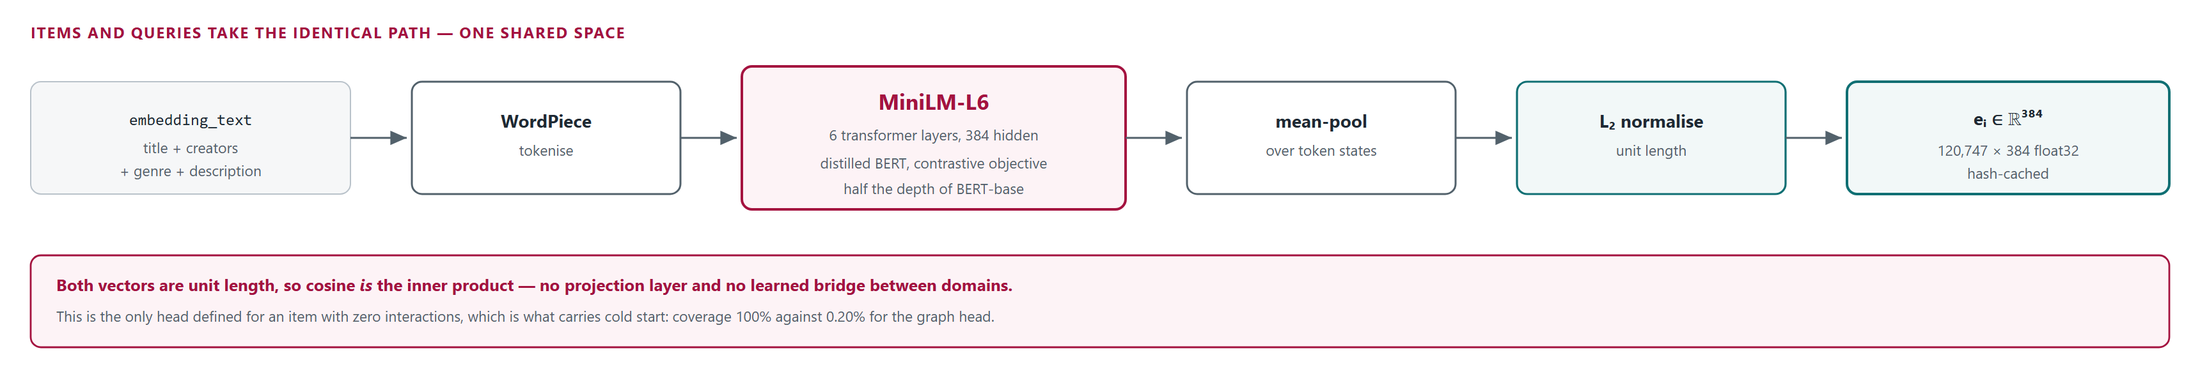
\includegraphics[width=\linewidth,height=3.4cm,keepaspectratio]{sbert}
\end{center}
\vspace{2mm}
\begin{columns}[T]
\column{0.485\textwidth}
\blk{Algorithm and equation}
{\scriptsize \texttt{all-MiniLM-L6-v2} --- a 6-layer distilled BERT, mean pooling over token states.
\[ \mathbf{e}_i = \frac{\mathrm{MeanPool}(\mathrm{MiniLM}(t_i))}{\lVert\cdot\rVert_2}, \quad
   S_{\mathit{sem}} = \mathbf{e}_i^{\top}\mathbf{q} \]
Both vectors are unit length, so cosine \emph{is} the inner product. The query takes the identical
path --- one shared space, no projection layer.}

\column{0.485\textwidth}
\blk{Measured}
\begin{tight}
  \item \textbf{120{,}747 $\times$ 384} float32; batch 256; hash-cached, so only changed rows
        re-encode.
  \item \textbf{Coverage 100\%} --- the only head defined at zero interactions, which is what
        carries cold start.
  \item 6 layers not 12, so the catalog encodes in one GPU pass and serving stays CPU-only.
\end{tight}
\end{columns}
\end{frame}

% ---------------------------------------------------------------------
\begin{frame}[shrink=15]{2. Model 2 --- LightGCN Graph Collaborative Filtering}
\framesubtitle{Algorithm $\cdot$ equation $\cdot$ measured result}
\vspace{1mm}
\begin{columns}[T]
\column{0.45\textwidth}
\blk{Algorithm}
{\scriptsize LightGCN (He et al., SIGIR 2020) --- a \emph{linear} convolution on the user--item
bipartite graph. Unlike NGCF there is \textbf{no feature transform and no nonlinearity}; the only
learned parameters are the layer-0 embeddings.}
\vspace{1.5mm}

\blk{Equations, as implemented}
{\scriptsize
With $\tilde{A} = D^{-1/2} A D^{-1/2}$, propagate and take the layer mean:
\[ \mathbf{E}^{(\ell)} = \tilde{A}\mathbf{E}^{(\ell-1)}, \quad
   \mathbf{E} = \tfrac{1}{L+1}\textstyle\sum_{\ell=0}^{L}\mathbf{E}^{(\ell)} \]
Score, and train by the BPR pairwise objective:
\[ \hat y_{ui} = \mathbf{e}_u^{\top}\mathbf{e}_i \]
\[ \mathcal{L} = -\!\sum \ln\sigma(\hat y_{ui}-\hat y_{uj}) + \lambda\lVert\mathbf{E}^{(0)}\rVert^2 \]}
\vspace{-1mm}
{\tiny\textbf{Config:} $d{=}64$, $L{=}3$, lr $10^{-3}$, decay $10^{-4}$, batch \textbf{4096},
60 epochs, seed 42, Kaggle T4.}

\column{0.52\textwidth}
\blk{Measured --- against a popularity control}
{\tiny
\renewcommand{\arraystretch}{1.15}
\begin{tabular}{L{1.4cm} l c c c c}
\toprule
\textbf{Domain} & \textbf{Model} & \textbf{R@20} & \textbf{N@20} & \textbf{MRR} & \textbf{Lift}\\
\midrule
Movies \& TV & LightGCN & \textbf{0.0288} & \textbf{0.0125} & \textbf{0.0080} & \\
             & popular  & 0.0182 & 0.0080 & 0.0052 & \textbf{1.59$\times$}\\
\midrule
Industrial   & LightGCN & \textbf{0.0326} & \textbf{0.0138} & \textbf{0.0087} & \\
             & popular  & 0.0264 & 0.0111 & 0.0070 & \textbf{1.24$\times$}\\
\midrule
Health       & LightGCN & 0.0121 & 0.0046 & 0.0025 & \\
             & popular  & \textbf{0.0221} & \textbf{0.0093} & \textbf{0.0059} & \textcolor{amritaMaroon}{\textbf{0.55$\times$}}\\
\bottomrule
\end{tabular}}\\[1.5mm]
{\tiny\textbf{Protocol.} Ratings $\geq 4$ as implicit positives; 10-core (Industrial keeps the
source 5-core floor); leave-last-out; 49{,}958 / 33{,}929 / 50{,}000 users evaluated.}\\[1.5mm]
{\tiny\textbf{$\mathtt{recall}=\mathtt{hit\_rate}$ is correct, not a bug:} leave-last-out gives one
relevant item, so Recall@$K \equiv$ HitRate@$K$. Check: $0.0288/20 = 0.00144$.}\\[1.5mm]
{\tiny\textcolor{amritaMaroon}{\textbf{Health regresses.}} BPR trains on the raw inner product, but
evaluation and serving both $L_2$-normalise and rank by cosine --- dividing by the \emph{item} norm
is not rank-preserving, and that norm carries the popularity prior.}
\end{columns}
\end{frame}

% ---------------------------------------------------------------------
%  PANEL RECOMMENDATION 1 -- NCF: position, architecture and plan
% ---------------------------------------------------------------------
\begin{frame}[shrink=15]{2. Panel Recommendation --- Neural Collaborative Filtering}
\framesubtitle{What NCF is, how it differs from LightGCN, and how we will test it}
\vspace{1mm}
\begin{columns}[T]
\column{0.475\textwidth}
\blk{What the panel asked for}
{\scriptsize NCF (He et al., WWW 2017) replaces the \emph{fixed} inner product with a \emph{learned}
similarity. NeuMF runs two towers and fuses them:
\[ \hat y^{\mathit{GMF}} = \mathbf{p}_u \odot \mathbf{q}_i, \quad
   \hat y^{\mathit{MLP}} = \phi_L(\cdots\phi_1([\mathbf{p}'_u \| \mathbf{q}'_i])) \]
\[ \hat y_{ui} = \sigma\big(\mathbf{h}^{\top}[\,\hat y^{\mathit{GMF}} \,\|\, \hat y^{\mathit{MLP}}\,]\big) \]
The MLP tower models \textbf{non-linear} interaction --- which our inner product cannot.}
\vspace{1.5mm}

\blk{How it differs from what we run}
\begin{tight}
  \item \textbf{LightGCN is graph-based:} it propagates over the bipartite graph, so a user is
        informed by items three hops away. \textbf{NCF has no graph} --- it learns a similarity on
        ids alone. They are complementary, not substitutes.
\end{tight}

\column{0.495\textwidth}
\vspace{-2mm}
\begin{center}
  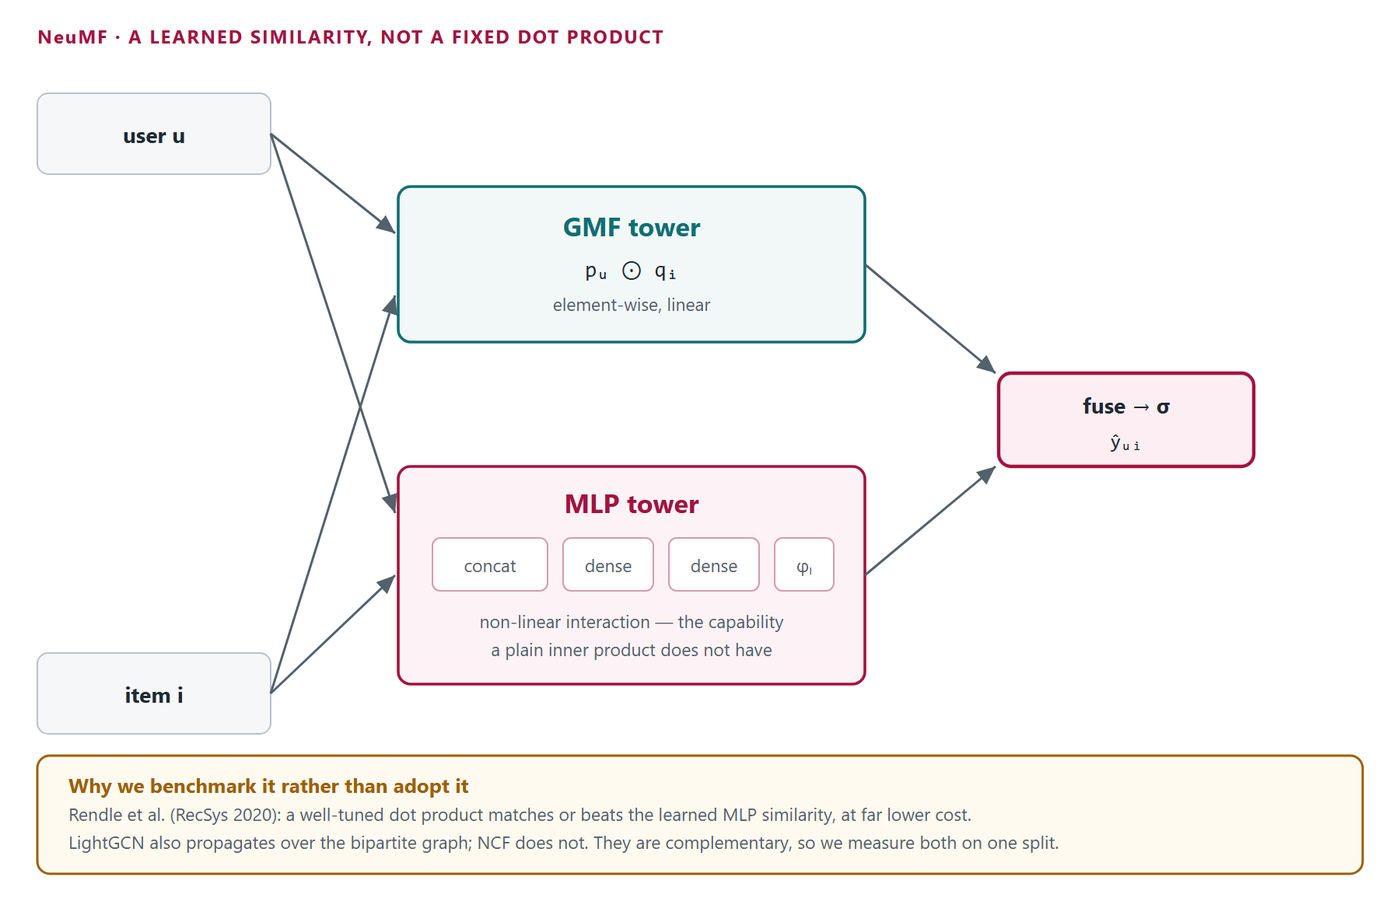
\includegraphics[width=\linewidth,height=4.9cm,keepaspectratio]{ncf}
\end{center}
\vspace{1mm}

\blk{Our position, and the plan}
\begin{tight}
  \item Rendle et al.\ (RecSys 2020) revisited this comparison and found a \textbf{well-tuned dot
        product matches or beats} the learned MLP, at far lower cost --- so we will run NeuMF as a
        \emph{measured baseline}, not adopt it as an assumed upgrade.
  \item The harness already runs three domains on fixed splits, so NeuMF slots in behind the same
        interface; then report popularity / LightGCN / NeuMF side by side.
\end{tight}
\end{columns}
\end{frame}

% ---------------------------------------------------------------------
\begin{frame}[shrink=15]{2. Model 3 --- Real-Time EMA User Vector}
\framesubtitle{Algorithm $\cdot$ equation $\cdot$ measured result}
\vspace{1mm}
\begin{columns}[T]
\column{0.515\textwidth}
\blk{Algorithm}
{\scriptsize A \textbf{signed, strength-scaled} exponential moving average in the same 384-d space
as the items. Not a plain average: a negative event pushes the user vector \emph{away} from the
item, and the step scales with how strong the event was.}
\vspace{1.5mm}

\blk{Equations, as implemented}
{\scriptsize
Event weight $w$: $+1.2$ complete, $+1.0$ like, $+0.6$ click, $+0.4$ view, $-1.0$ skip; a rating
$v$ maps to $(v-3)/2$. Then with $\alpha = 0.25$:
\[ d=\operatorname{sign}(w),\ \ s=\min(|w|,1),\ \ \eta=\operatorname{clip}(\alpha s,0,1) \]
\[ \mathbf{u}_{t+1} = \frac{(1-\eta)\mathbf{u}_t + \eta\,d\,\mathbf{e}_i}{\lVert\cdot\rVert_2},
   \ \ S_{\mathit{ema}} = \mathbf{u}_t^{\top}\mathbf{e}_i \]}

\column{0.46\textwidth}
\vspace{-3mm}
\begin{center}
  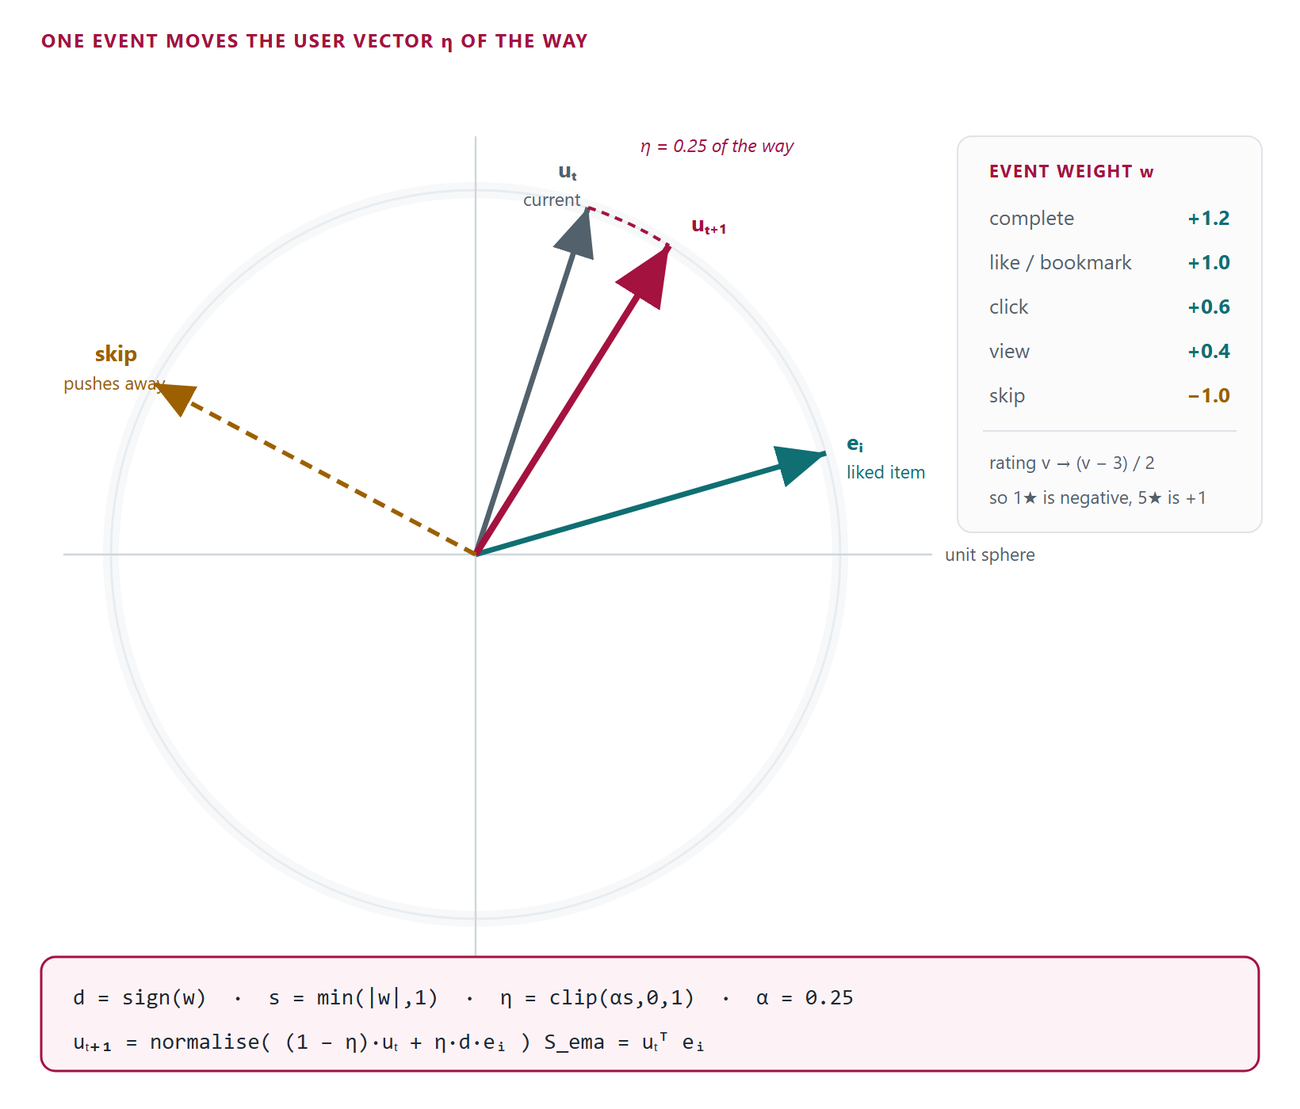
\includegraphics[width=\linewidth,height=5.5cm,keepaspectratio]{ema}
\end{center}
\vspace{1mm}

\blk{Measured}
\begin{tight}
  \item \textbf{39.0\,$\mu$s} per update, \textbf{16.7\,$\mu$s} per score (1{,}000 ops, 384-d).
  \item Against \textbf{hours} for a retrain --- five orders of magnitude. This is the "real-time"
        in the project title, as a number.
  \item \textbf{Limitation:} no session boundary or time decay, so one misclick persists.
\end{tight}
\end{columns}
\end{frame}

% ---------------------------------------------------------------------
\begin{frame}[shrink=15]{2. Model 4 --- Knowledge-Graph Overlap Head}
\framesubtitle{Algorithm $\cdot$ equation $\cdot$ measured result}
\vspace{1mm}
\begin{columns}[T]
\column{0.47\textwidth}
\blk{Algorithm and equation}
{\scriptsize A \textbf{zero-parameter set-overlap scorer} over shared entity namespaces. Nothing is
trained, so nothing drifts --- and it is defined precisely where the graph model is not. With
$T(i)$ the token set over \{title, description, creators, categories, type\}:
\[ S_{\mathit{kg}} = \min\!\left(1,\ \frac{|T(q)\cap T(i)|}{\max(3,|T(q)|)}\right) \]
The $\max(3,\cdot)$ floor stops a one-word query scoring 1.0 on one incidental match.}
\vspace{1.5mm}

\blk{Measured}
\begin{tight}
  \item Mean \textbf{KG@5 $=$ 0.892} over 8 scenarios; \textbf{0.667} on both named-entity queries,
        where dense retrieval smears.
  \item \textbf{Coverage 100\%} --- it reads metadata, not behaviour.
\end{tight}

\column{0.50\textwidth}
\vspace{-3mm}
\begin{center}
  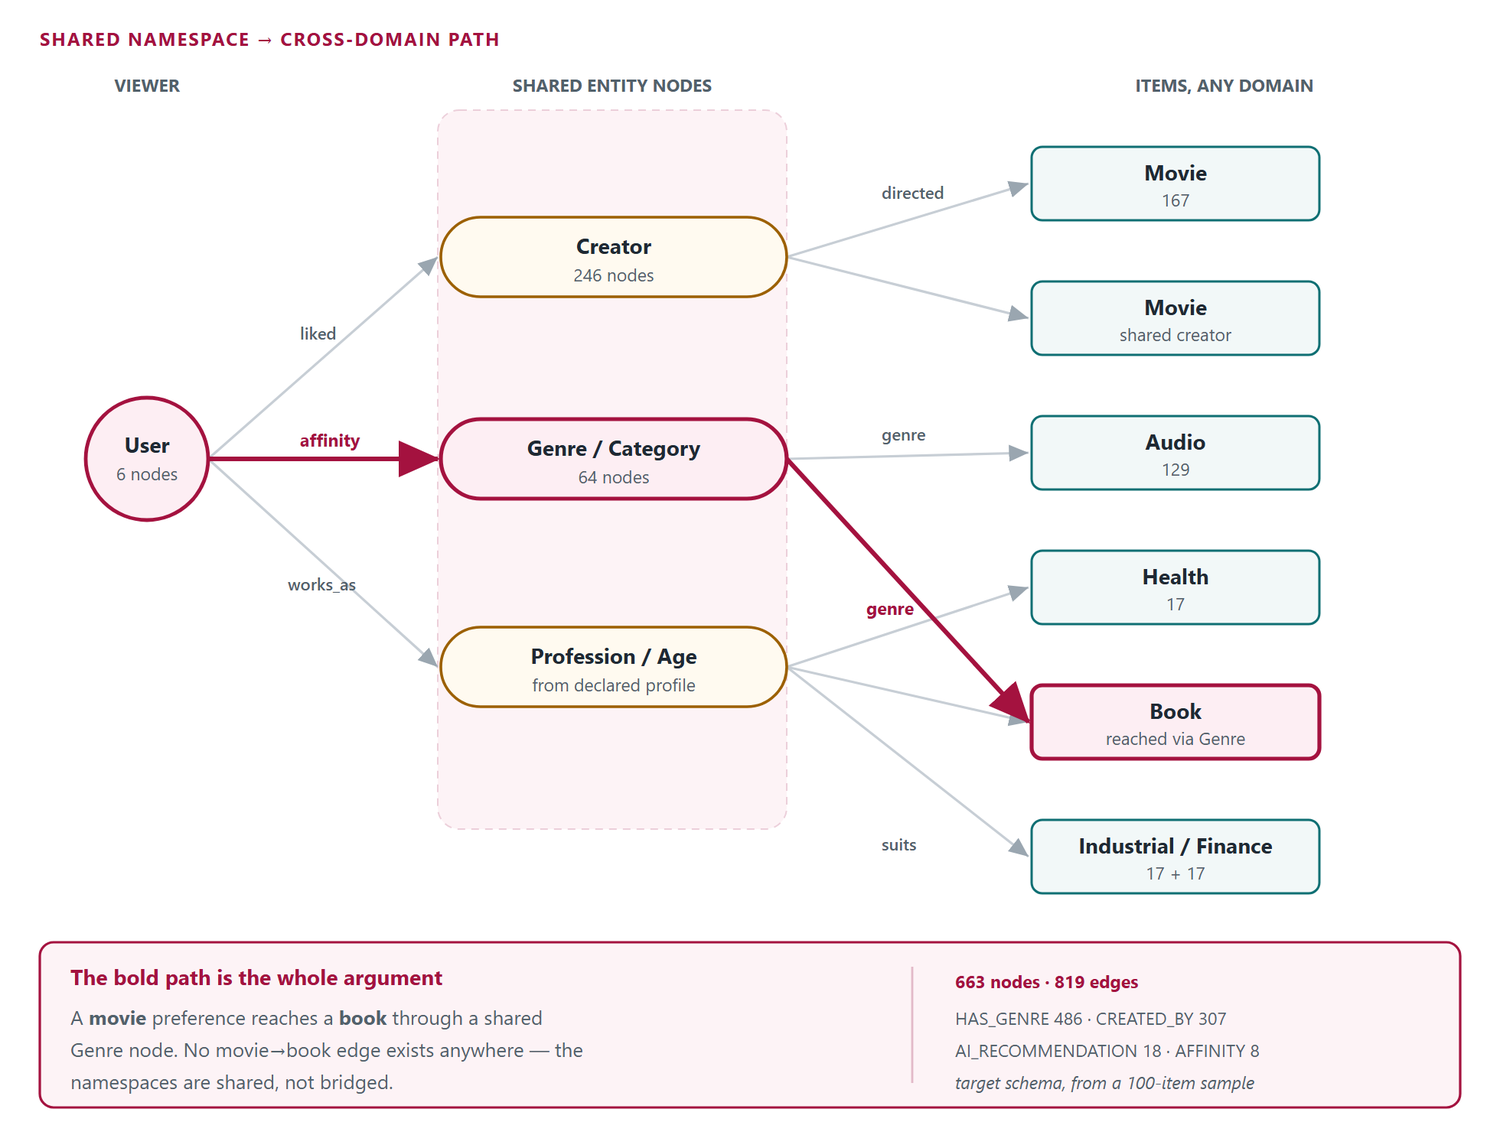
\includegraphics[width=\linewidth,height=5.7cm,keepaspectratio]{kg}
\end{center}
\vspace{1mm}

{\scriptsize\textcolor{amritaMaroon}{\textbf{Bold path:}} a \emph{movie} preference reaches a
\emph{book} through a shared Genre node --- no movie-to-book edge exists anywhere.}\\[1mm]
{\tiny\textbf{Scope.} At request time this is the overlap function above; the 663-node figure is the
\emph{target schema} from a 100-item example, not a runtime graph. Neo4j is Review 3.}
\end{columns}
\end{frame}

% ---------------------------------------------------------------------
\begin{frame}[shrink=15]{2. Model 5 --- Profile Head and the Eligibility Gate}
\framesubtitle{Algorithm $\cdot$ equation $\cdot$ measured result}
\vspace{1mm}
\begin{columns}[T]
\column{0.53\textwidth}
\blk{Profile head --- a score}
{\footnotesize A \textbf{weighted term matcher} against the declared profile; avoid-terms subtract
at nearly twice the weight of a positive match.
\[ S_{\mathit{profile}} = \operatorname{clip}\big(0.16|P\cap i| - 0.25|A\cap i| + 0.15\cdot\mathbf{1}[\tau_i \in \Pi]\big) \]}
\vspace{-3mm}
{\scriptsize $P$ = interests $\cup$ likes $\cup$ skills $\cup$ role $\cup$ age terms; \ $A$ = avoid
terms; \ $\Pi$ = preferred types; clipped to $[-1,1]$.}
\vspace{3mm}

\blk{Eligibility --- a predicate, not a score}
{\footnotesize
\[ \mathrm{elig}(i\,|\,c) = \mathbf{1}\big[a_{\mathit{eff}} \geq \mathrm{minage}(i)\big] \wedge \mathbf{1}\big[\tau_i \in \mathcal{T}(d)\big] \]
Compiled \emph{into} the Qdrant query, so an ineligible item is never retrieved, never scored, and
cannot be promoted back by any head.}
\vspace{2mm}

{\footnotesize\textbf{Fail-closed.} No age supplied caps at teen, not adult. Unknown metadata falls
back to the content-type default, never to unrestricted. Health and finance are \textbf{discovery
only, never advice}.}

\column{0.445\textwidth}
\vspace{-2mm}
\begin{center}
  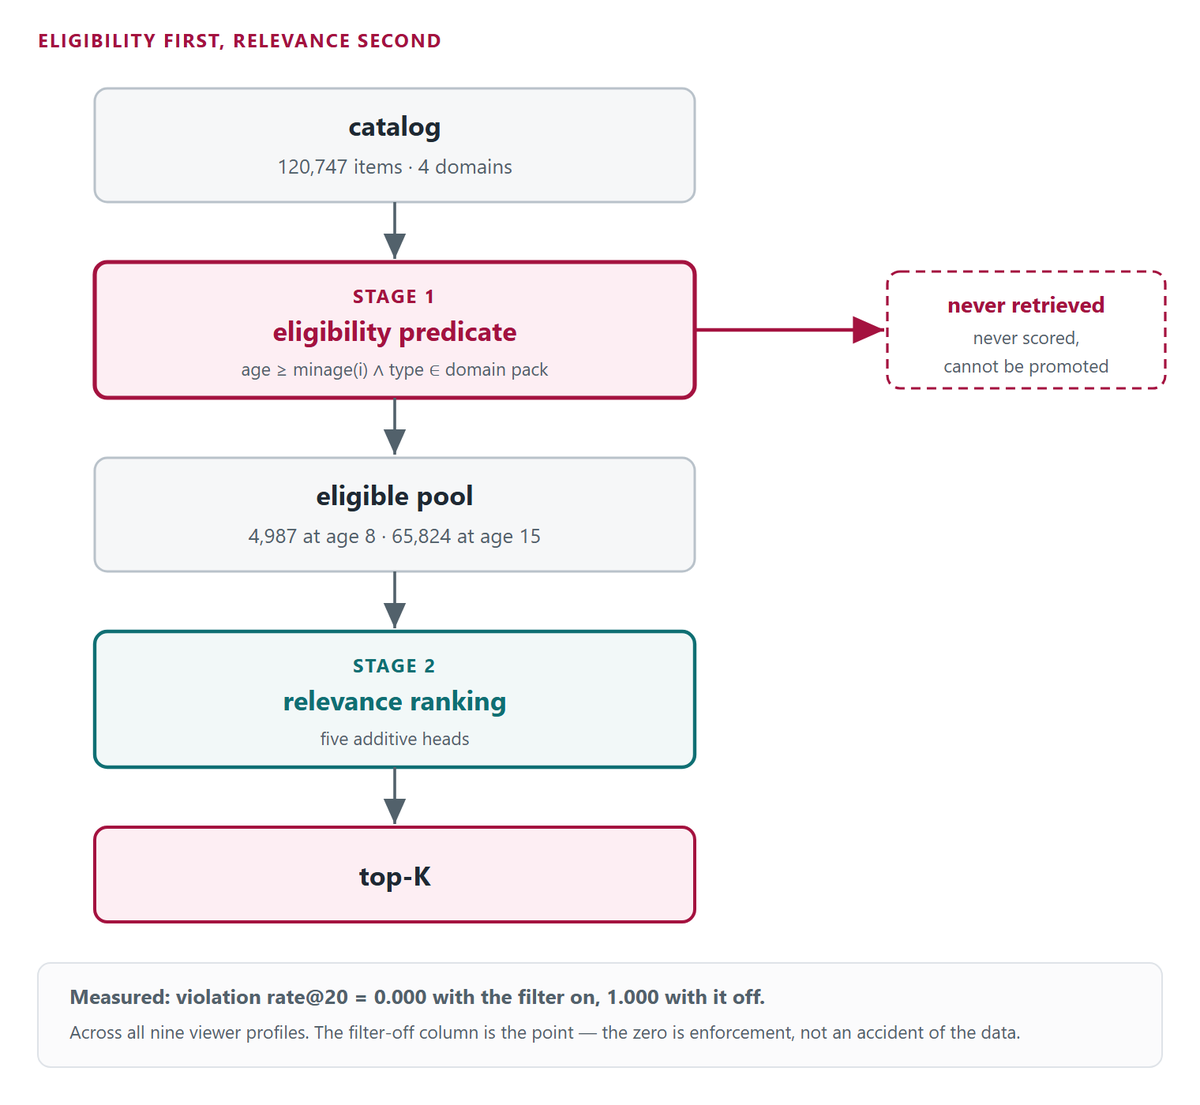
\includegraphics[width=\linewidth,height=5.9cm,keepaspectratio]{gate}
\end{center}
\vspace{2mm}
\blk{Measured}
\begin{tight}
  \item Mean \textbf{profile@5 $=$ 0.957}; \textbf{8 of 8} scenarios fully profile-positive.
  \item Violations \textbf{0.000} on, \textbf{1.000} off, across \textbf{9} viewer profiles.
\end{tight}
\end{columns}
\end{frame}
 from 2_presentation.tex
%
%  Every card carries the same four things in the same order:
%     ALGORITHM  --  what it is, by name
%     EQUATION   --  what the code computes
%     DIAGRAM    --  the mechanism, drawn
%     MEASURED   --  a number from this repository
%
%  HEIGHT BUDGET -- READ THIS BEFORE ADDING A LINE.
%  A 16:9 frame gives ~6.8cm of body once title, subtitle and footline
%  are paid for. That is about 20 lines at \scriptsize, 27 at \tiny.
%  A display equation \[..\] costs ~3 lines.
%
%  Every card carries [shrink=15]: beamer measures the frame and scales
%  it down ONLY if it would overflow, up to 15%. A frame that already
%  fits is untouched. This is a SAFETY NET, not a licence to overfill --
%  past 15% the content runs off the bottom edge silently, exactly as it
%  did before. If you add an equation, delete a bullet to pay for it.
%
%  Overleaf prints "Overfull \vbox" for any frame that needed shrinking;
%  that warning is the signal to cut a line, not to raise the 15%.
%
%  All figures measured from the repository, 14 Sep 2026.
% =====================================================================

% ---------------------------------------------------------------------
\begin{frame}[shrink=15]{2. Model Inventory --- Five Scoring Heads and One Gate}
\framesubtitle{Each is a different model class, defined where the others are not}
\vspace{1mm}
\begin{center}
{\scriptsize
\renewcommand{\arraystretch}{1.22}
\begin{tabular}{c L{2.5cm} L{3.9cm} c c c}
\toprule
\textbf{Head} & \textbf{Model class} & \textbf{What it computes} & \textbf{Range} & \textbf{Cov.} & \textbf{Wt.}\\
\midrule
$S_{\mathit{sem}}$     & Transformer encoder   & Cosine to a 384-d sentence embedding & $[-1,1]$ & \textbf{100\%} & $1.00$\\
$S_{\mathit{graph}}$   & Graph neural net (CF) & Inner product of LightGCN embeddings & $[-1,1]$ & \textcolor{amritaMaroon}{\textbf{0.20\%}} & $0.20$\\
$S_{\mathit{ema}}$     & Online moving average & Cosine to the live user vector       & $[-1,1]$ & \textbf{100\%} & $0.15$\\
$S_{\mathit{kg}}$      & Set overlap, 0 params & Query / entity token overlap         & $[0,1]$  & \textbf{100\%} & $0.08$\\
$S_{\mathit{profile}}$ & Weighted term matcher & Declared-profile alignment           & $[-1,1]$ & \textbf{100\%} & $0.10$\\
\midrule
\textit{gate} & \textit{Hard predicate} & \textit{May this viewer see this item at all?} & $\{0,1\}$ & \textbf{100\%} & \textit{---}\\
\bottomrule
\end{tabular}}
\end{center}
\vspace{1mm}
{\scriptsize
\[ S(q,u,i) = S_{\mathit{sem}} + 0.20\,S_{\mathit{graph}} + 0.15\,S_{\mathit{ema}} + 0.08\,S_{\mathit{kg}} + 0.10\,S_{\mathit{profile}} \]}
\vspace{-3mm}
{\scriptsize\textbf{Why coverage is the column that matters.} The graph head is our strongest signal
and is defined for \textbf{0.20\%} of the catalog; every other head is defined everywhere. That is
why the blend is additive with a dominant semantic term rather than a learned gate --- a missing
head must degrade the ranking, never break it.}
\end{frame}

% ---------------------------------------------------------------------
\begin{frame}[shrink=15]{2. Model 1 --- SBERT Semantic Encoder}
\framesubtitle{Algorithm $\cdot$ equation $\cdot$ measured result}
\vspace{1mm}
\begin{center}
  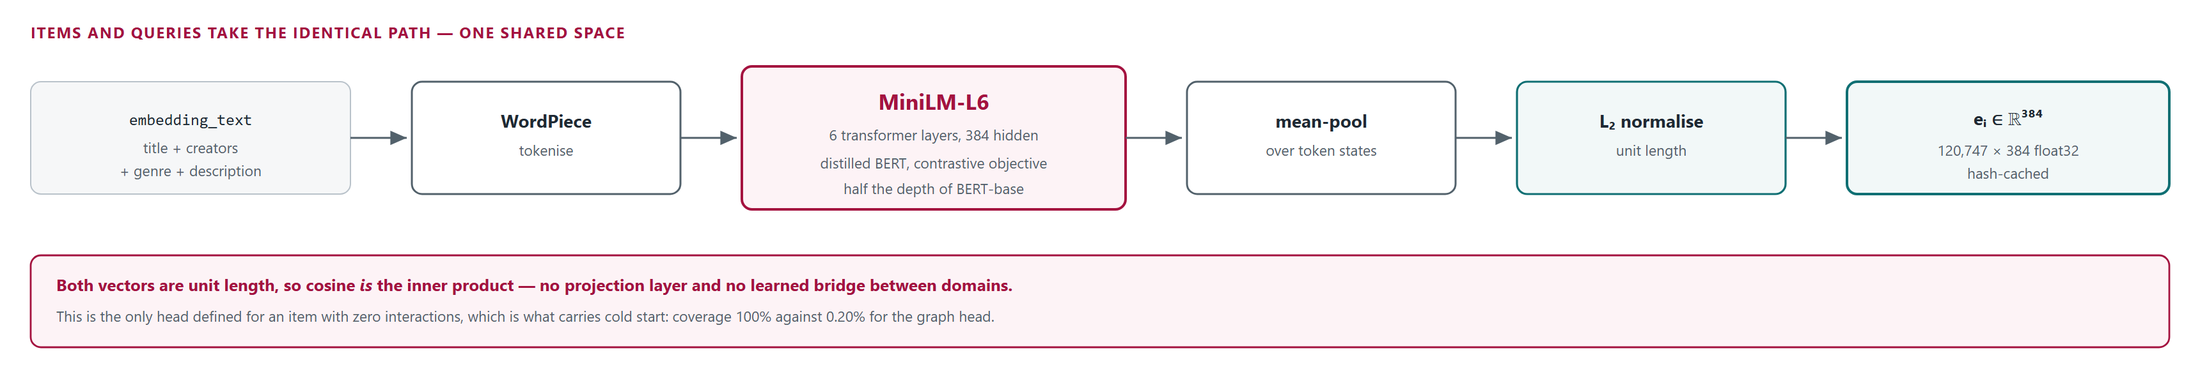
\includegraphics[width=\linewidth,height=3.4cm,keepaspectratio]{sbert}
\end{center}
\vspace{2mm}
\begin{columns}[T]
\column{0.485\textwidth}
\blk{Algorithm and equation}
{\scriptsize \texttt{all-MiniLM-L6-v2} --- a 6-layer distilled BERT, mean pooling over token states.
\[ \mathbf{e}_i = \frac{\mathrm{MeanPool}(\mathrm{MiniLM}(t_i))}{\lVert\cdot\rVert_2}, \quad
   S_{\mathit{sem}} = \mathbf{e}_i^{\top}\mathbf{q} \]
Both vectors are unit length, so cosine \emph{is} the inner product. The query takes the identical
path --- one shared space, no projection layer.}

\column{0.485\textwidth}
\blk{Measured}
\begin{tight}
  \item \textbf{120{,}747 $\times$ 384} float32; batch 256; hash-cached, so only changed rows
        re-encode.
  \item \textbf{Coverage 100\%} --- the only head defined at zero interactions, which is what
        carries cold start.
  \item 6 layers not 12, so the catalog encodes in one GPU pass and serving stays CPU-only.
\end{tight}
\end{columns}
\end{frame}

% ---------------------------------------------------------------------
\begin{frame}[shrink=15]{2. Model 2 --- LightGCN Graph Collaborative Filtering}
\framesubtitle{Algorithm $\cdot$ equation $\cdot$ measured result}
\vspace{1mm}
\begin{columns}[T]
\column{0.45\textwidth}
\blk{Algorithm}
{\scriptsize LightGCN (He et al., SIGIR 2020) --- a \emph{linear} convolution on the user--item
bipartite graph. Unlike NGCF there is \textbf{no feature transform and no nonlinearity}; the only
learned parameters are the layer-0 embeddings.}
\vspace{1.5mm}

\blk{Equations, as implemented}
{\scriptsize
With $\tilde{A} = D^{-1/2} A D^{-1/2}$, propagate and take the layer mean:
\[ \mathbf{E}^{(\ell)} = \tilde{A}\mathbf{E}^{(\ell-1)}, \quad
   \mathbf{E} = \tfrac{1}{L+1}\textstyle\sum_{\ell=0}^{L}\mathbf{E}^{(\ell)} \]
Score, and train by the BPR pairwise objective:
\[ \hat y_{ui} = \mathbf{e}_u^{\top}\mathbf{e}_i \]
\[ \mathcal{L} = -\!\sum \ln\sigma(\hat y_{ui}-\hat y_{uj}) + \lambda\lVert\mathbf{E}^{(0)}\rVert^2 \]}
\vspace{-1mm}
{\tiny\textbf{Config:} $d{=}64$, $L{=}3$, lr $10^{-3}$, decay $10^{-4}$, batch \textbf{4096},
60 epochs, seed 42, Kaggle T4.}

\column{0.52\textwidth}
\blk{Measured --- against a popularity control}
{\tiny
\renewcommand{\arraystretch}{1.15}
\begin{tabular}{L{1.4cm} l c c c c}
\toprule
\textbf{Domain} & \textbf{Model} & \textbf{R@20} & \textbf{N@20} & \textbf{MRR} & \textbf{Lift}\\
\midrule
Movies \& TV & LightGCN & \textbf{0.0288} & \textbf{0.0125} & \textbf{0.0080} & \\
             & popular  & 0.0182 & 0.0080 & 0.0052 & \textbf{1.59$\times$}\\
\midrule
Industrial   & LightGCN & \textbf{0.0326} & \textbf{0.0138} & \textbf{0.0087} & \\
             & popular  & 0.0264 & 0.0111 & 0.0070 & \textbf{1.24$\times$}\\
\midrule
Health       & LightGCN & 0.0121 & 0.0046 & 0.0025 & \\
             & popular  & \textbf{0.0221} & \textbf{0.0093} & \textbf{0.0059} & \textcolor{amritaMaroon}{\textbf{0.55$\times$}}\\
\bottomrule
\end{tabular}}\\[1.5mm]
{\tiny\textbf{Protocol.} Ratings $\geq 4$ as implicit positives; 10-core (Industrial keeps the
source 5-core floor); leave-last-out; 49{,}958 / 33{,}929 / 50{,}000 users evaluated.}\\[1.5mm]
{\tiny\textbf{$\mathtt{recall}=\mathtt{hit\_rate}$ is correct, not a bug:} leave-last-out gives one
relevant item, so Recall@$K \equiv$ HitRate@$K$. Check: $0.0288/20 = 0.00144$.}\\[1.5mm]
{\tiny\textcolor{amritaMaroon}{\textbf{Health regresses.}} BPR trains on the raw inner product, but
evaluation and serving both $L_2$-normalise and rank by cosine --- dividing by the \emph{item} norm
is not rank-preserving, and that norm carries the popularity prior.}
\end{columns}
\end{frame}

% ---------------------------------------------------------------------
%  PANEL RECOMMENDATION 1 -- NCF: position, architecture and plan
% ---------------------------------------------------------------------
\begin{frame}[shrink=15]{2. Panel Recommendation --- Neural Collaborative Filtering}
\framesubtitle{What NCF is, how it differs from LightGCN, and how we will test it}
\vspace{1mm}
\begin{columns}[T]
\column{0.475\textwidth}
\blk{What the panel asked for}
{\scriptsize NCF (He et al., WWW 2017) replaces the \emph{fixed} inner product with a \emph{learned}
similarity. NeuMF runs two towers and fuses them:
\[ \hat y^{\mathit{GMF}} = \mathbf{p}_u \odot \mathbf{q}_i, \quad
   \hat y^{\mathit{MLP}} = \phi_L(\cdots\phi_1([\mathbf{p}'_u \| \mathbf{q}'_i])) \]
\[ \hat y_{ui} = \sigma\big(\mathbf{h}^{\top}[\,\hat y^{\mathit{GMF}} \,\|\, \hat y^{\mathit{MLP}}\,]\big) \]
The MLP tower models \textbf{non-linear} interaction --- which our inner product cannot.}
\vspace{1.5mm}

\blk{How it differs from what we run}
\begin{tight}
  \item \textbf{LightGCN is graph-based:} it propagates over the bipartite graph, so a user is
        informed by items three hops away. \textbf{NCF has no graph} --- it learns a similarity on
        ids alone. They are complementary, not substitutes.
\end{tight}

\column{0.495\textwidth}
\vspace{-2mm}
\begin{center}
  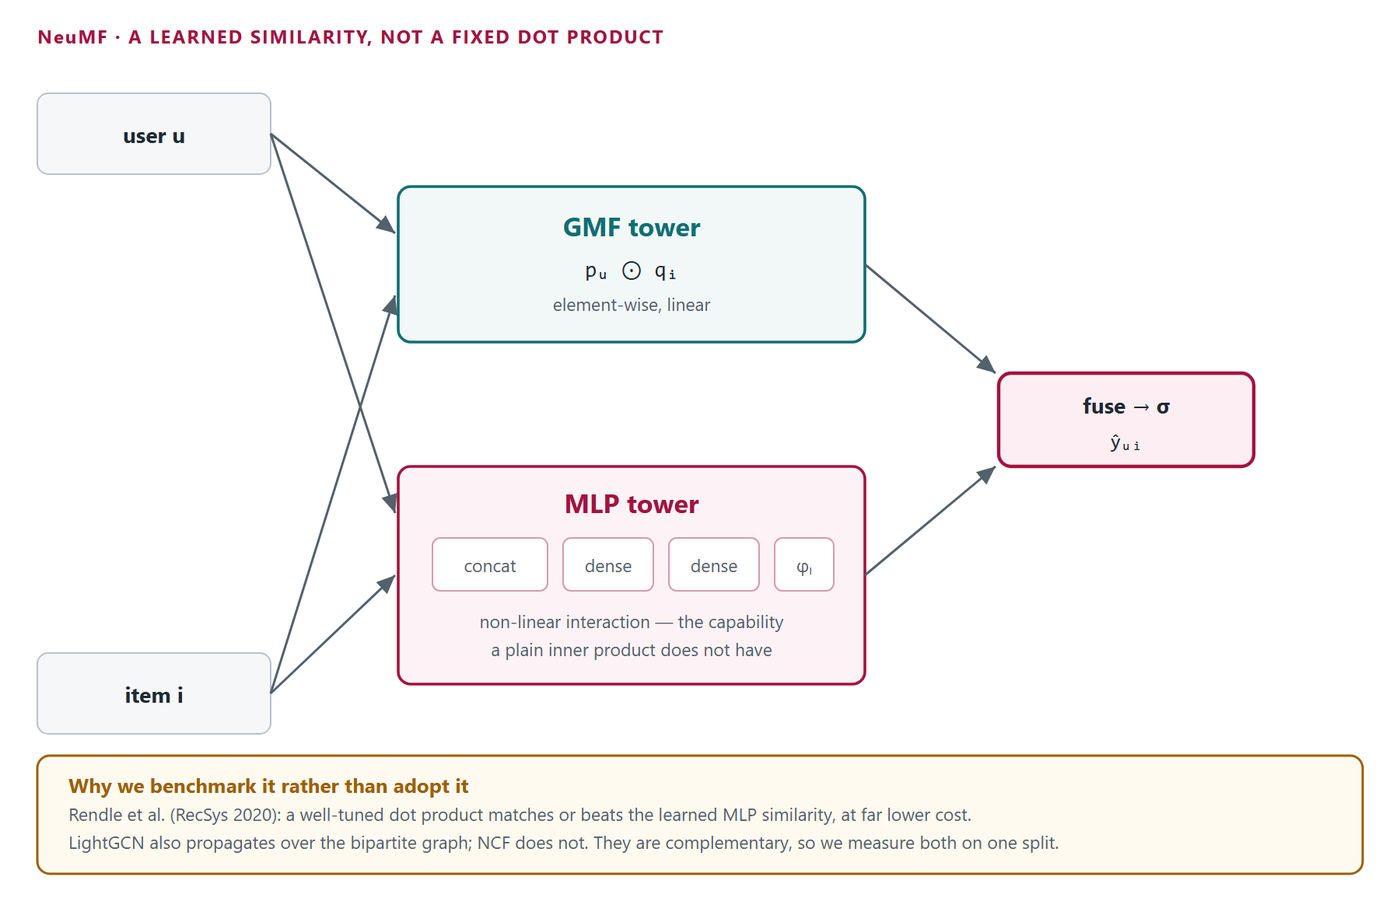
\includegraphics[width=\linewidth,height=4.9cm,keepaspectratio]{ncf}
\end{center}
\vspace{1mm}

\blk{Our position, and the plan}
\begin{tight}
  \item Rendle et al.\ (RecSys 2020) revisited this comparison and found a \textbf{well-tuned dot
        product matches or beats} the learned MLP, at far lower cost --- so we will run NeuMF as a
        \emph{measured baseline}, not adopt it as an assumed upgrade.
  \item The harness already runs three domains on fixed splits, so NeuMF slots in behind the same
        interface; then report popularity / LightGCN / NeuMF side by side.
\end{tight}
\end{columns}
\end{frame}

% ---------------------------------------------------------------------
\begin{frame}[shrink=15]{2. Model 3 --- Real-Time EMA User Vector}
\framesubtitle{Algorithm $\cdot$ equation $\cdot$ measured result}
\vspace{1mm}
\begin{columns}[T]
\column{0.515\textwidth}
\blk{Algorithm}
{\scriptsize A \textbf{signed, strength-scaled} exponential moving average in the same 384-d space
as the items. Not a plain average: a negative event pushes the user vector \emph{away} from the
item, and the step scales with how strong the event was.}
\vspace{1.5mm}

\blk{Equations, as implemented}
{\scriptsize
Event weight $w$: $+1.2$ complete, $+1.0$ like, $+0.6$ click, $+0.4$ view, $-1.0$ skip; a rating
$v$ maps to $(v-3)/2$. Then with $\alpha = 0.25$:
\[ d=\operatorname{sign}(w),\ \ s=\min(|w|,1),\ \ \eta=\operatorname{clip}(\alpha s,0,1) \]
\[ \mathbf{u}_{t+1} = \frac{(1-\eta)\mathbf{u}_t + \eta\,d\,\mathbf{e}_i}{\lVert\cdot\rVert_2},
   \ \ S_{\mathit{ema}} = \mathbf{u}_t^{\top}\mathbf{e}_i \]}

\column{0.46\textwidth}
\vspace{-3mm}
\begin{center}
  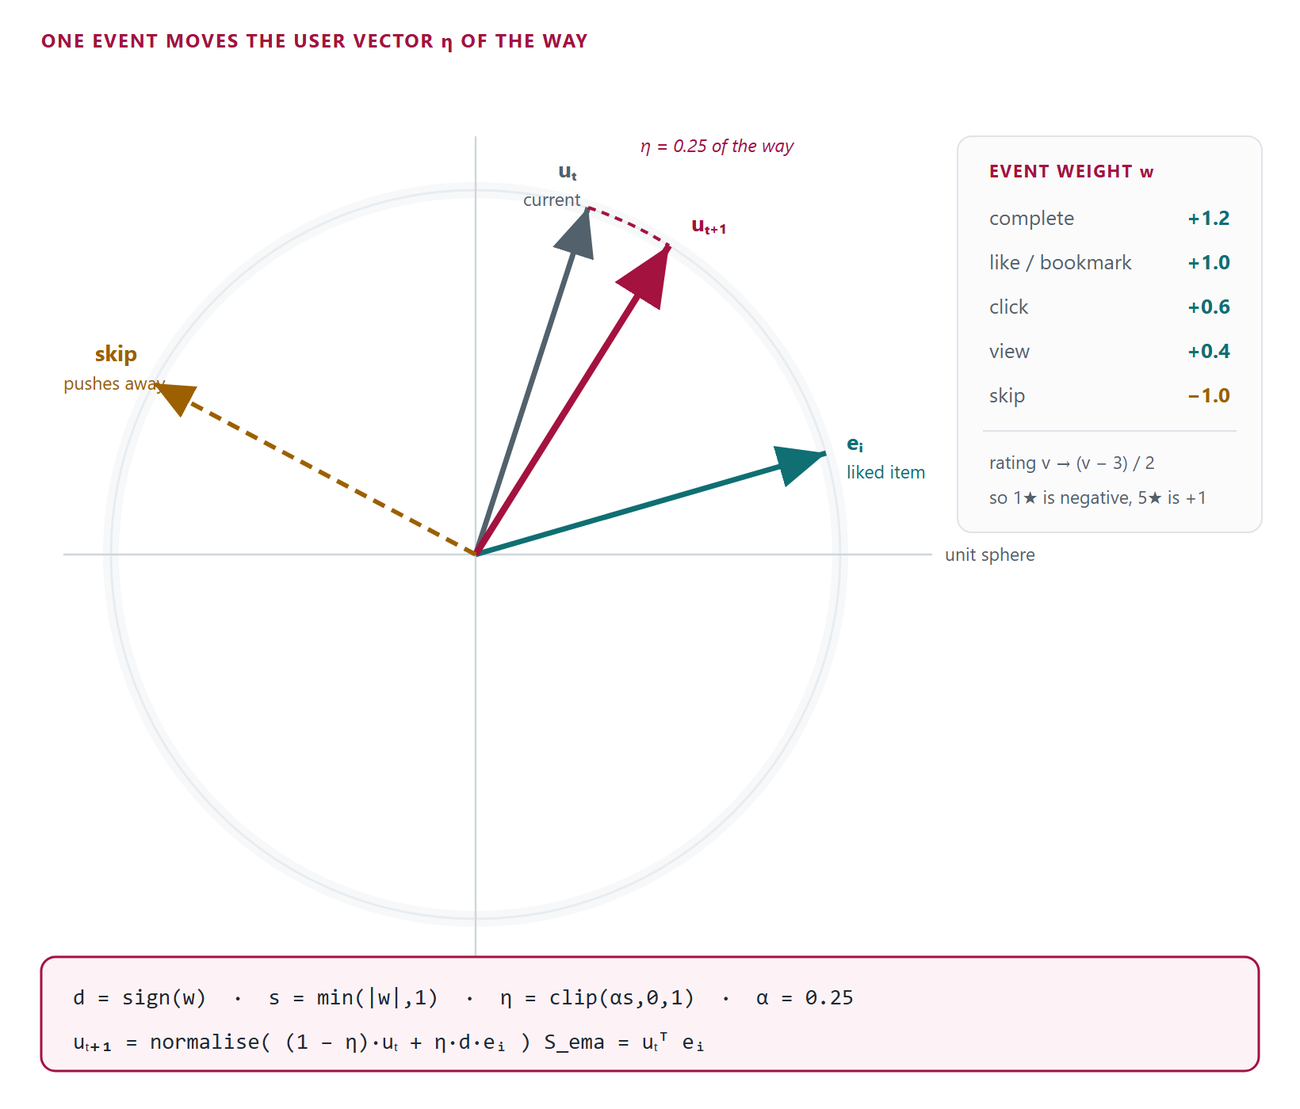
\includegraphics[width=\linewidth,height=5.5cm,keepaspectratio]{ema}
\end{center}
\vspace{1mm}

\blk{Measured}
\begin{tight}
  \item \textbf{39.0\,$\mu$s} per update, \textbf{16.7\,$\mu$s} per score (1{,}000 ops, 384-d).
  \item Against \textbf{hours} for a retrain --- five orders of magnitude. This is the "real-time"
        in the project title, as a number.
  \item \textbf{Limitation:} no session boundary or time decay, so one misclick persists.
\end{tight}
\end{columns}
\end{frame}

% ---------------------------------------------------------------------
\begin{frame}[shrink=15]{2. Model 4 --- Knowledge-Graph Overlap Head}
\framesubtitle{Algorithm $\cdot$ equation $\cdot$ measured result}
\vspace{1mm}
\begin{columns}[T]
\column{0.47\textwidth}
\blk{Algorithm and equation}
{\scriptsize A \textbf{zero-parameter set-overlap scorer} over shared entity namespaces. Nothing is
trained, so nothing drifts --- and it is defined precisely where the graph model is not. With
$T(i)$ the token set over \{title, description, creators, categories, type\}:
\[ S_{\mathit{kg}} = \min\!\left(1,\ \frac{|T(q)\cap T(i)|}{\max(3,|T(q)|)}\right) \]
The $\max(3,\cdot)$ floor stops a one-word query scoring 1.0 on one incidental match.}
\vspace{1.5mm}

\blk{Measured}
\begin{tight}
  \item Mean \textbf{KG@5 $=$ 0.892} over 8 scenarios; \textbf{0.667} on both named-entity queries,
        where dense retrieval smears.
  \item \textbf{Coverage 100\%} --- it reads metadata, not behaviour.
\end{tight}

\column{0.50\textwidth}
\vspace{-3mm}
\begin{center}
  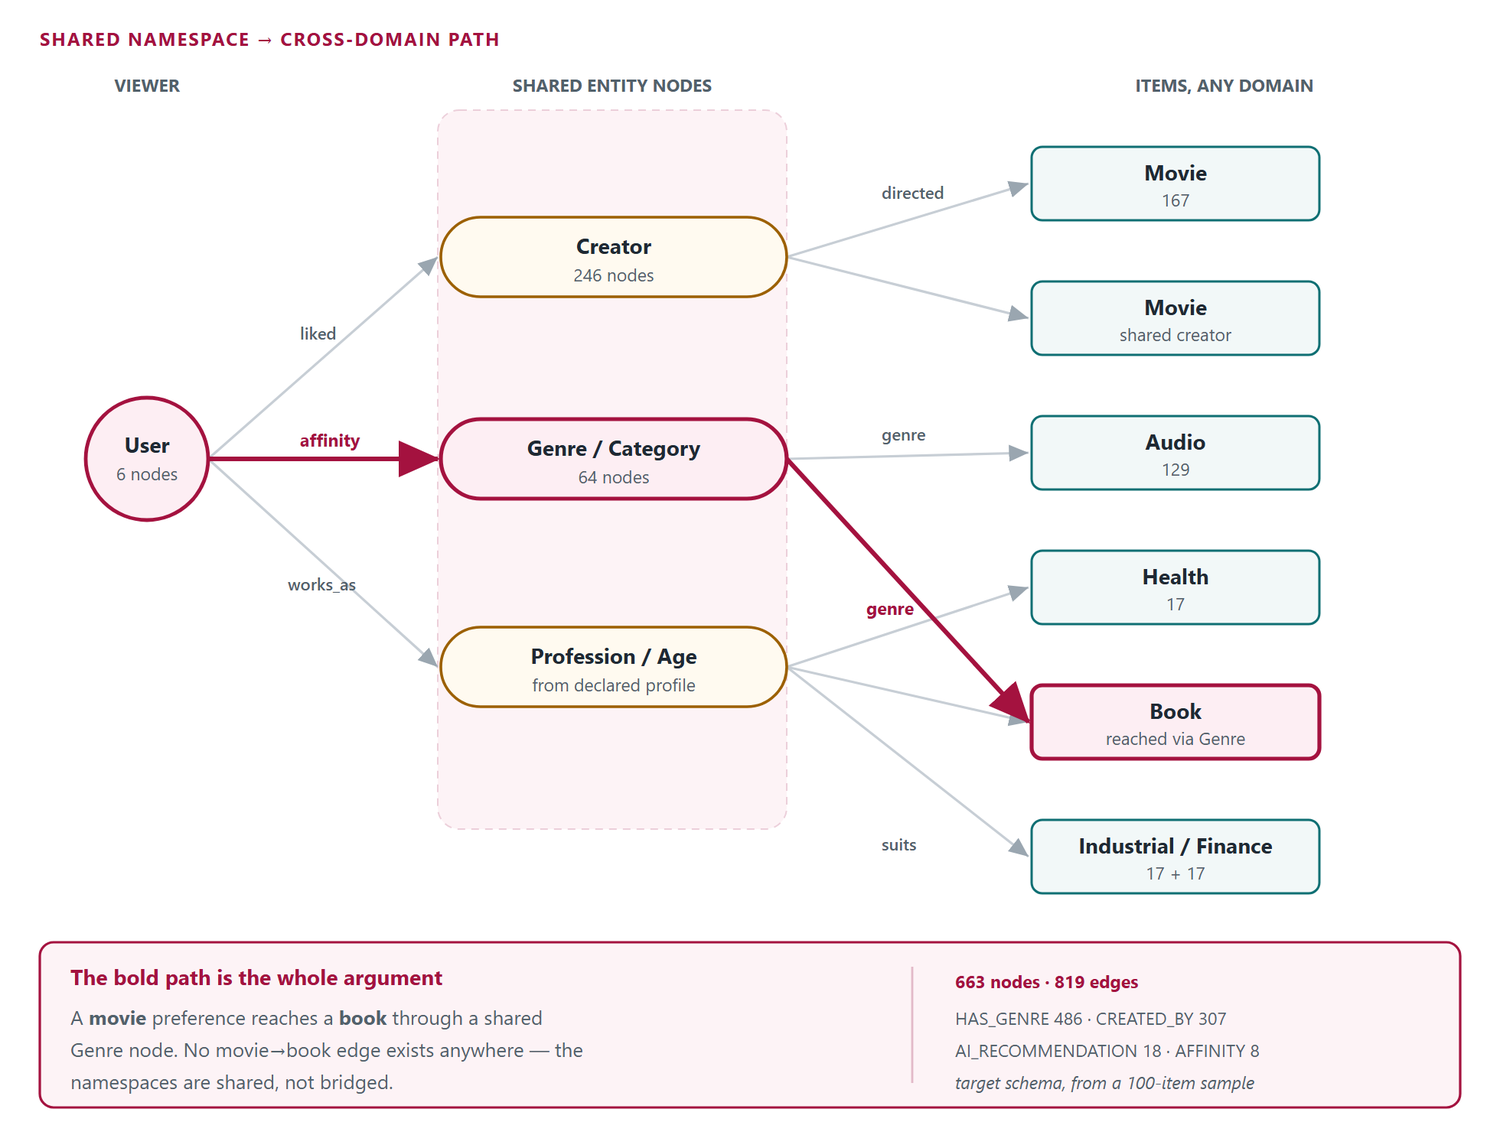
\includegraphics[width=\linewidth,height=5.7cm,keepaspectratio]{kg}
\end{center}
\vspace{1mm}

{\scriptsize\textcolor{amritaMaroon}{\textbf{Bold path:}} a \emph{movie} preference reaches a
\emph{book} through a shared Genre node --- no movie-to-book edge exists anywhere.}\\[1mm]
{\tiny\textbf{Scope.} At request time this is the overlap function above; the 663-node figure is the
\emph{target schema} from a 100-item example, not a runtime graph. Neo4j is Review 3.}
\end{columns}
\end{frame}

% ---------------------------------------------------------------------
\begin{frame}[shrink=15]{2. Model 5 --- Profile Head and the Eligibility Gate}
\framesubtitle{Algorithm $\cdot$ equation $\cdot$ measured result}
\vspace{1mm}
\begin{columns}[T]
\column{0.53\textwidth}
\blk{Profile head --- a score}
{\footnotesize A \textbf{weighted term matcher} against the declared profile; avoid-terms subtract
at nearly twice the weight of a positive match.
\[ S_{\mathit{profile}} = \operatorname{clip}\big(0.16|P\cap i| - 0.25|A\cap i| + 0.15\cdot\mathbf{1}[\tau_i \in \Pi]\big) \]}
\vspace{-3mm}
{\scriptsize $P$ = interests $\cup$ likes $\cup$ skills $\cup$ role $\cup$ age terms; \ $A$ = avoid
terms; \ $\Pi$ = preferred types; clipped to $[-1,1]$.}
\vspace{3mm}

\blk{Eligibility --- a predicate, not a score}
{\footnotesize
\[ \mathrm{elig}(i\,|\,c) = \mathbf{1}\big[a_{\mathit{eff}} \geq \mathrm{minage}(i)\big] \wedge \mathbf{1}\big[\tau_i \in \mathcal{T}(d)\big] \]
Compiled \emph{into} the Qdrant query, so an ineligible item is never retrieved, never scored, and
cannot be promoted back by any head.}
\vspace{2mm}

{\footnotesize\textbf{Fail-closed.} No age supplied caps at teen, not adult. Unknown metadata falls
back to the content-type default, never to unrestricted. Health and finance are \textbf{discovery
only, never advice}.}

\column{0.445\textwidth}
\vspace{-2mm}
\begin{center}
  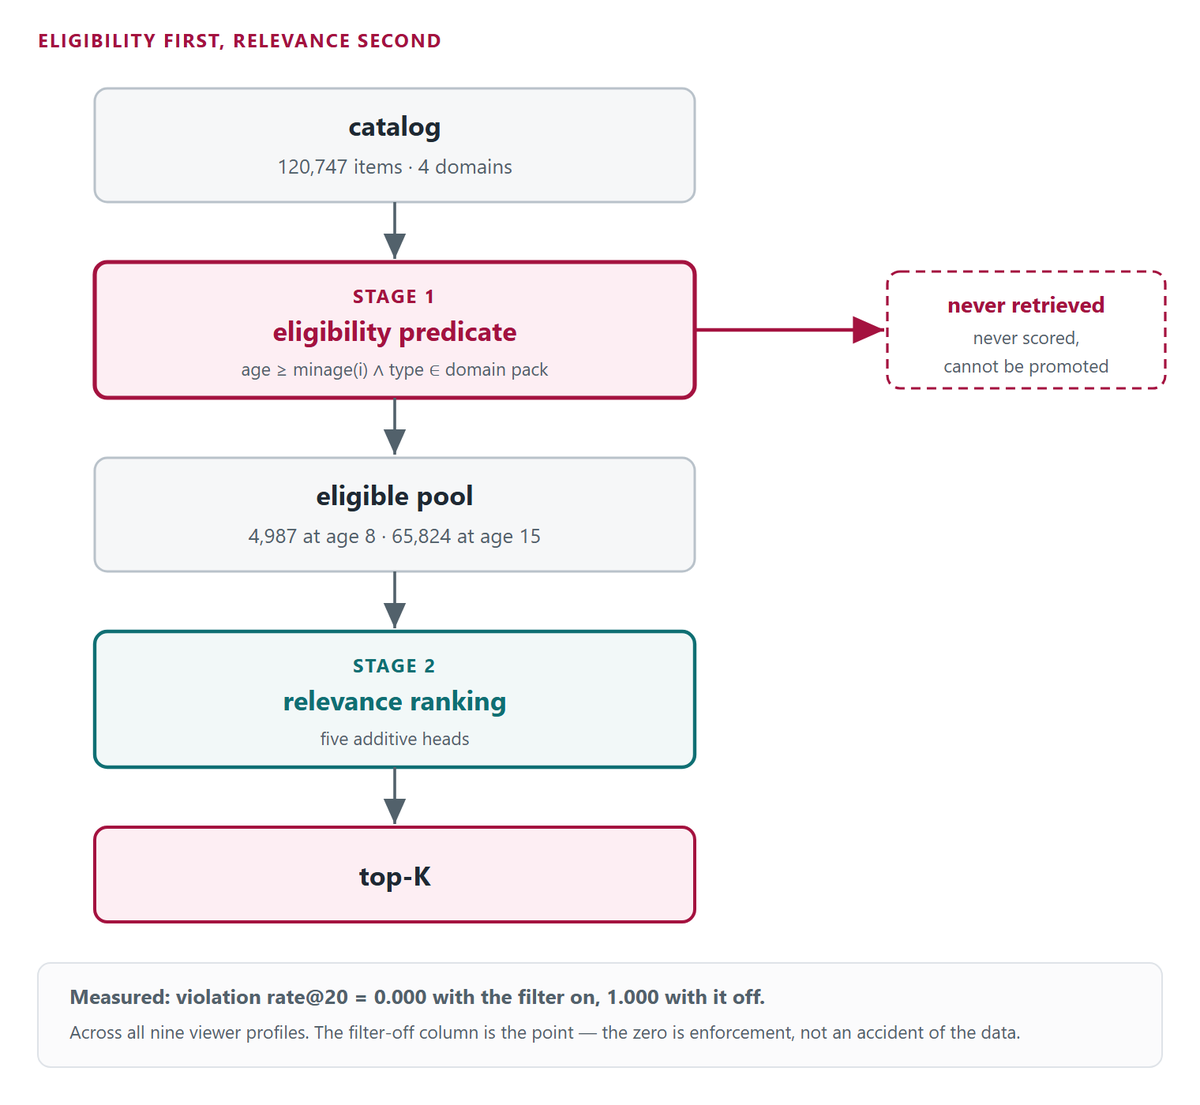
\includegraphics[width=\linewidth,height=5.9cm,keepaspectratio]{gate}
\end{center}
\vspace{2mm}
\blk{Measured}
\begin{tight}
  \item Mean \textbf{profile@5 $=$ 0.957}; \textbf{8 of 8} scenarios fully profile-positive.
  \item Violations \textbf{0.000} on, \textbf{1.000} off, across \textbf{9} viewer profiles.
\end{tight}
\end{columns}
\end{frame}
